\documentclass[english]{article}
\usepackage[utf8]{inputenc}
\usepackage[T1]{fontenc}
\usepackage{stix2}
\usepackage{babel}
\usepackage[section]{placeins}
\usepackage{flafter}
\usepackage{comment}
\usepackage{svg}
\usepackage{caption, booktabs}
\usepackage{amsmath}
\usepackage{graphicx}
\usepackage{fancyhdr}
% \usepackage[disable]{todonotes}
\usepackage{todonotes}
\usepackage{units}
\usepackage[left=2cm,right=4cm,top=2cm,bottom=2cm]{geometry}
\usepackage[
colorlinks=true,
	citecolor=black,
  urlcolor=black,
	linkcolor=black
]{hyperref}
%\newcommand{\scidatalogo}{
\includegraphics[height=36pt]{SciData_logo.jpg}}
\newcommand{\scidatalogo}{}
\pagestyle{fancy}
\fancyhf{}
\renewcommand{\headrulewidth}{0pt}
\setlength{\headheight}{40pt}
\lhead{\textsc{\scidatalogo}}
\usepackage{natbib}

% \usepackage{helvet}

% \renewcommand{\familydefault}{\sfdefault}

\begin{document}
\newcommand{\aoBodyAll}{66}
\newcommand{\aoBodyI}{6}
\newcommand{\aoBodyII}{12}
\newcommand{\aoBodyIII}{7}
\newcommand{\aoBodyIV}{12}
\newcommand{\aoBodyV}{2}
\newcommand{\aoBodyVI}{9}
\newcommand{\aoBodyVII}{13}
\newcommand{\aoBodyVIII}{5}

\newcommand{\aoBpartAll}{69}
\newcommand{\aoBpartI}{9}
\newcommand{\aoBpartII}{8}
\newcommand{\aoBpartIII}{6}
\newcommand{\aoBpartIV}{13}
\newcommand{\aoBpartV}{5}
\newcommand{\aoBpartVI}{7}
\newcommand{\aoBpartVII}{11}
\newcommand{\aoBpartVIII}{10}

\newcommand{\aoFaheadAll}{83}
\newcommand{\aoFaheadI}{12}
\newcommand{\aoFaheadII}{11}
\newcommand{\aoFaheadIII}{10}
\newcommand{\aoFaheadIV}{5}
\newcommand{\aoFaheadV}{9}
\newcommand{\aoFaheadVI}{13}
\newcommand{\aoFaheadVII}{12}
\newcommand{\aoFaheadVIII}{11}

\newcommand{\aoFgadlrdiffAll}{180133}
\newcommand{\aoFgadlrdiffI}{22574}
\newcommand{\aoFgadlrdiffII}{22075}
\newcommand{\aoFgadlrdiffIII}{21925}
\newcommand{\aoFgadlrdiffIV}{24425}
\newcommand{\aoFgadlrdiffV}{23125}
\newcommand{\aoFgadlrdiffVI}{21975}
\newcommand{\aoFgadlrdiffVII}{27175}
\newcommand{\aoFgadlrdiffVIII}{16859}

\newcommand{\aoFgadrmsAll}{180133}
\newcommand{\aoFgadrmsI}{22574}
\newcommand{\aoFgadrmsII}{22075}
\newcommand{\aoFgadrmsIII}{21925}
\newcommand{\aoFgadrmsIV}{24425}
\newcommand{\aoFgadrmsV}{23125}
\newcommand{\aoFgadrmsVI}{21975}
\newcommand{\aoFgadrmsVII}{27175}
\newcommand{\aoFgadrmsVIII}{16859}

\newcommand{\aoFurnAll}{50}
\newcommand{\aoFurnI}{8}
\newcommand{\aoFurnII}{5}
\newcommand{\aoFurnIII}{2}
\newcommand{\aoFurnIV}{5}
\newcommand{\aoFurnV}{7}
\newcommand{\aoFurnVI}{10}
\newcommand{\aoFurnVII}{7}
\newcommand{\aoFurnVIII}{6}

\newcommand{\aoGeoAll}{125}
\newcommand{\aoGeoI}{16}
\newcommand{\aoGeoII}{17}
\newcommand{\aoGeoIII}{11}
\newcommand{\aoGeoIV}{32}
\newcommand{\aoGeoV}{0}
\newcommand{\aoGeoVI}{15}
\newcommand{\aoGeoVII}{18}
\newcommand{\aoGeoVIII}{16}

\newcommand{\aoGroomAll}{105}
\newcommand{\aoGroomI}{12}
\newcommand{\aoGroomII}{11}
\newcommand{\aoGroomIII}{8}
\newcommand{\aoGroomIV}{5}
\newcommand{\aoGroomV}{8}
\newcommand{\aoGroomVI}{25}
\newcommand{\aoGroomVII}{28}
\newcommand{\aoGroomVIII}{8}

\newcommand{\aoObjAll}{284}
\newcommand{\aoObjI}{39}
\newcommand{\aoObjII}{34}
\newcommand{\aoObjIII}{27}
\newcommand{\aoObjIV}{44}
\newcommand{\aoObjV}{29}
\newcommand{\aoObjVI}{42}
\newcommand{\aoObjVII}{32}
\newcommand{\aoObjVIII}{37}

\newcommand{\aoSenewAll}{86}
\newcommand{\aoSenewI}{11}
\newcommand{\aoSenewII}{15}
\newcommand{\aoSenewIII}{12}
\newcommand{\aoSenewIV}{4}
\newcommand{\aoSenewV}{15}
\newcommand{\aoSenewVI}{10}
\newcommand{\aoSenewVII}{16}
\newcommand{\aoSenewVIII}{3}

\newcommand{\aoSeoldAll}{37}
\newcommand{\aoSeoldI}{2}
\newcommand{\aoSeoldII}{5}
\newcommand{\aoSeoldIII}{1}
\newcommand{\aoSeoldIV}{4}
\newcommand{\aoSeoldV}{2}
\newcommand{\aoSeoldVI}{9}
\newcommand{\aoSeoldVII}{8}
\newcommand{\aoSeoldVIII}{6}

\newcommand{\aoSexfAll}{108}
\newcommand{\aoSexfI}{14}
\newcommand{\aoSexfII}{22}
\newcommand{\aoSexfIII}{6}
\newcommand{\aoSexfIV}{6}
\newcommand{\aoSexfV}{13}
\newcommand{\aoSexfVI}{10}
\newcommand{\aoSexfVII}{23}
\newcommand{\aoSexfVIII}{14}

\newcommand{\aoSexmAll}{403}
\newcommand{\aoSexmI}{41}
\newcommand{\aoSexmII}{68}
\newcommand{\aoSexmIII}{38}
\newcommand{\aoSexmIV}{102}
\newcommand{\aoSexmV}{45}
\newcommand{\aoSexmVI}{42}
\newcommand{\aoSexmVII}{42}
\newcommand{\aoSexmVIII}{25}

\newcommand{\aoSexuAll}{17}
\newcommand{\aoSexuI}{0}
\newcommand{\aoSexuII}{3}
\newcommand{\aoSexuIII}{1}
\newcommand{\aoSexuIV}{2}
\newcommand{\aoSexuV}{3}
\newcommand{\aoSexuVI}{1}
\newcommand{\aoSexuVII}{5}
\newcommand{\aoSexuVIII}{2}

\newcommand{\aoVlochAll}{89}
\newcommand{\aoVlochI}{10}
\newcommand{\aoVlochII}{31}
\newcommand{\aoVlochIII}{2}
\newcommand{\aoVlochIV}{23}
\newcommand{\aoVlochV}{4}
\newcommand{\aoVlochVI}{18}
\newcommand{\aoVlochVII}{1}
\newcommand{\aoVnocutAll}{148}
\newcommand{\aoVnocutI}{30}
\newcommand{\aoVnocutII}{13}
\newcommand{\aoVnocutIII}{21}
\newcommand{\aoVnocutIV}{15}
\newcommand{\aoVnocutV}{27}
\newcommand{\aoVnocutVI}{9}
\newcommand{\aoVnocutVII}{17}
\newcommand{\aoVnocutVIII}{16}

\newcommand{\aoVpenewAll}{386}
\newcommand{\aoVpenewI}{31}
\newcommand{\aoVpenewII}{38}
\newcommand{\aoVpenewIII}{72}
\newcommand{\aoVpenewIV}{90}
\newcommand{\aoVpenewV}{89}
\newcommand{\aoVpenewVI}{33}
\newcommand{\aoVpenewVII}{24}
\newcommand{\aoVpenewVIII}{9}

\newcommand{\aoVpeoldAll}{208}
\newcommand{\aoVpeoldI}{25}
\newcommand{\aoVpeoldII}{61}
\newcommand{\aoVpeoldIII}{13}
\newcommand{\aoVpeoldIV}{1}
\newcommand{\aoVpeoldV}{32}
\newcommand{\aoVpeoldVI}{29}
\newcommand{\aoVpeoldVII}{47}
\newcommand{\aoVsenewAll}{96}
\newcommand{\aoVsenewI}{11}
\newcommand{\aoVsenewII}{14}
\newcommand{\aoVsenewIII}{17}
\newcommand{\aoVsenewIV}{4}
\newcommand{\aoVsenewV}{17}
\newcommand{\aoVsenewVI}{9}
\newcommand{\aoVsenewVII}{21}
\newcommand{\aoVsenewVIII}{3}

\newcommand{\aoVseoldAll}{90}
\newcommand{\aoVseoldI}{7}
\newcommand{\aoVseoldII}{11}
\newcommand{\aoVseoldIII}{3}
\newcommand{\aoVseoldIV}{7}
\newcommand{\aoVseoldV}{7}
\newcommand{\aoVseoldVI}{23}
\newcommand{\aoVseoldVII}{15}
\newcommand{\aoVseoldVIII}{17}


\newcommand{\avBodyAll}{66}
\newcommand{\avBodyI}{6}
\newcommand{\avBodyII}{12}
\newcommand{\avBodyIII}{7}
\newcommand{\avBodyIV}{12}
\newcommand{\avBodyV}{2}
\newcommand{\avBodyVI}{9}
\newcommand{\avBodyVII}{13}
\newcommand{\avBodyVIII}{5}

\newcommand{\avBpartAll}{69}
\newcommand{\avBpartI}{9}
\newcommand{\avBpartII}{8}
\newcommand{\avBpartIII}{6}
\newcommand{\avBpartIV}{13}
\newcommand{\avBpartV}{5}
\newcommand{\avBpartVI}{7}
\newcommand{\avBpartVII}{11}
\newcommand{\avBpartVIII}{10}

\newcommand{\avFaheadAll}{83}
\newcommand{\avFaheadI}{12}
\newcommand{\avFaheadII}{11}
\newcommand{\avFaheadIII}{10}
\newcommand{\avFaheadIV}{5}
\newcommand{\avFaheadV}{9}
\newcommand{\avFaheadVI}{13}
\newcommand{\avFaheadVII}{12}
\newcommand{\avFaheadVIII}{11}

\newcommand{\avFgavgerlrAll}{180783}
\newcommand{\avFgavgerlrI}{22656}
\newcommand{\avFgavgerlrII}{22158}
\newcommand{\avFgavgerlrIII}{22008}
\newcommand{\avFgavgerlrIV}{24507}
\newcommand{\avFgavgerlrV}{23208}
\newcommand{\avFgavgerlrVI}{22057}
\newcommand{\avFgavgerlrVII}{27208}
\newcommand{\avFgavgerlrVIII}{16981}

\newcommand{\avFgavgerlrdiffAll}{180759}
\newcommand{\avFgavgerlrdiffI}{22653}
\newcommand{\avFgavgerlrdiffII}{22155}
\newcommand{\avFgavgerlrdiffIII}{22005}
\newcommand{\avFgavgerlrdiffIV}{24504}
\newcommand{\avFgavgerlrdiffV}{23205}
\newcommand{\avFgavgerlrdiffVI}{22054}
\newcommand{\avFgavgerlrdiffVII}{27205}
\newcommand{\avFgavgerlrdiffVIII}{16978}

\newcommand{\avFgavgermlAll}{180783}
\newcommand{\avFgavgermlI}{22656}
\newcommand{\avFgavgermlII}{22158}
\newcommand{\avFgavgermlIII}{22008}
\newcommand{\avFgavgermlIV}{24507}
\newcommand{\avFgavgermlV}{23208}
\newcommand{\avFgavgermlVI}{22057}
\newcommand{\avFgavgermlVII}{27208}
\newcommand{\avFgavgermlVIII}{16981}

\newcommand{\avFgavgerpdAll}{180783}
\newcommand{\avFgavgerpdI}{22656}
\newcommand{\avFgavgerpdII}{22158}
\newcommand{\avFgavgerpdIII}{22008}
\newcommand{\avFgavgerpdIV}{24507}
\newcommand{\avFgavgerpdV}{23208}
\newcommand{\avFgavgerpdVI}{22057}
\newcommand{\avFgavgerpdVII}{27208}
\newcommand{\avFgavgerpdVIII}{16981}

\newcommand{\avFgavgerrmsAll}{180759}
\newcommand{\avFgavgerrmsI}{22653}
\newcommand{\avFgavgerrmsII}{22155}
\newcommand{\avFgavgerrmsIII}{22005}
\newcommand{\avFgavgerrmsIV}{24504}
\newcommand{\avFgavgerrmsV}{23205}
\newcommand{\avFgavgerrmsVI}{22054}
\newcommand{\avFgavgerrmsVII}{27205}
\newcommand{\avFgavgerrmsVIII}{16978}

\newcommand{\avFgavgerudAll}{180783}
\newcommand{\avFgavgerudI}{22656}
\newcommand{\avFgavgerudII}{22158}
\newcommand{\avFgavgerudIII}{22008}
\newcommand{\avFgavgerudIV}{24507}
\newcommand{\avFgavgerudV}{23208}
\newcommand{\avFgavgerudVI}{22057}
\newcommand{\avFgavgerudVII}{27208}
\newcommand{\avFgavgerudVIII}{16981}

\newcommand{\avFurnAll}{50}
\newcommand{\avFurnI}{8}
\newcommand{\avFurnII}{5}
\newcommand{\avFurnIII}{2}
\newcommand{\avFurnIV}{5}
\newcommand{\avFurnV}{7}
\newcommand{\avFurnVI}{10}
\newcommand{\avFurnVII}{7}
\newcommand{\avFurnVIII}{6}

\newcommand{\avGeoAll}{125}
\newcommand{\avGeoI}{16}
\newcommand{\avGeoII}{17}
\newcommand{\avGeoIII}{11}
\newcommand{\avGeoIV}{32}
\newcommand{\avGeoV}{0}
\newcommand{\avGeoVI}{15}
\newcommand{\avGeoVII}{18}
\newcommand{\avGeoVIII}{16}

\newcommand{\avGroomAll}{105}
\newcommand{\avGroomI}{12}
\newcommand{\avGroomII}{11}
\newcommand{\avGroomIII}{8}
\newcommand{\avGroomIV}{5}
\newcommand{\avGroomV}{8}
\newcommand{\avGroomVI}{25}
\newcommand{\avGroomVII}{28}
\newcommand{\avGroomVIII}{8}

\newcommand{\avObjAll}{284}
\newcommand{\avObjI}{39}
\newcommand{\avObjII}{34}
\newcommand{\avObjIII}{27}
\newcommand{\avObjIV}{44}
\newcommand{\avObjV}{29}
\newcommand{\avObjVI}{42}
\newcommand{\avObjVII}{32}
\newcommand{\avObjVIII}{37}

\newcommand{\avSenewAll}{86}
\newcommand{\avSenewI}{11}
\newcommand{\avSenewII}{15}
\newcommand{\avSenewIII}{12}
\newcommand{\avSenewIV}{4}
\newcommand{\avSenewV}{15}
\newcommand{\avSenewVI}{10}
\newcommand{\avSenewVII}{16}
\newcommand{\avSenewVIII}{3}

\newcommand{\avSeoldAll}{37}
\newcommand{\avSeoldI}{2}
\newcommand{\avSeoldII}{5}
\newcommand{\avSeoldIII}{1}
\newcommand{\avSeoldIV}{4}
\newcommand{\avSeoldV}{2}
\newcommand{\avSeoldVI}{9}
\newcommand{\avSeoldVII}{8}
\newcommand{\avSeoldVIII}{6}

\newcommand{\avSexfAll}{108}
\newcommand{\avSexfI}{14}
\newcommand{\avSexfII}{22}
\newcommand{\avSexfIII}{6}
\newcommand{\avSexfIV}{6}
\newcommand{\avSexfV}{13}
\newcommand{\avSexfVI}{10}
\newcommand{\avSexfVII}{23}
\newcommand{\avSexfVIII}{14}

\newcommand{\avSexmAll}{403}
\newcommand{\avSexmI}{41}
\newcommand{\avSexmII}{68}
\newcommand{\avSexmIII}{38}
\newcommand{\avSexmIV}{102}
\newcommand{\avSexmV}{45}
\newcommand{\avSexmVI}{42}
\newcommand{\avSexmVII}{42}
\newcommand{\avSexmVIII}{25}

\newcommand{\avSexuAll}{17}
\newcommand{\avSexuI}{0}
\newcommand{\avSexuII}{3}
\newcommand{\avSexuIII}{1}
\newcommand{\avSexuIV}{2}
\newcommand{\avSexuV}{3}
\newcommand{\avSexuVI}{1}
\newcommand{\avSexuVII}{5}
\newcommand{\avSexuVIII}{2}

\newcommand{\avVlochAll}{89}
\newcommand{\avVlochI}{10}
\newcommand{\avVlochII}{31}
\newcommand{\avVlochIII}{2}
\newcommand{\avVlochIV}{23}
\newcommand{\avVlochV}{4}
\newcommand{\avVlochVI}{18}
\newcommand{\avVlochVII}{1}
\newcommand{\avVnocutAll}{148}
\newcommand{\avVnocutI}{30}
\newcommand{\avVnocutII}{13}
\newcommand{\avVnocutIII}{21}
\newcommand{\avVnocutIV}{15}
\newcommand{\avVnocutV}{27}
\newcommand{\avVnocutVI}{9}
\newcommand{\avVnocutVII}{17}
\newcommand{\avVnocutVIII}{16}

\newcommand{\avVpenewAll}{386}
\newcommand{\avVpenewI}{31}
\newcommand{\avVpenewII}{38}
\newcommand{\avVpenewIII}{72}
\newcommand{\avVpenewIV}{90}
\newcommand{\avVpenewV}{89}
\newcommand{\avVpenewVI}{33}
\newcommand{\avVpenewVII}{24}
\newcommand{\avVpenewVIII}{9}

\newcommand{\avVpeoldAll}{208}
\newcommand{\avVpeoldI}{25}
\newcommand{\avVpeoldII}{61}
\newcommand{\avVpeoldIII}{13}
\newcommand{\avVpeoldIV}{1}
\newcommand{\avVpeoldV}{32}
\newcommand{\avVpeoldVI}{29}
\newcommand{\avVpeoldVII}{47}
\newcommand{\avVsenewAll}{96}
\newcommand{\avVsenewI}{11}
\newcommand{\avVsenewII}{14}
\newcommand{\avVsenewIII}{17}
\newcommand{\avVsenewIV}{4}
\newcommand{\avVsenewV}{17}
\newcommand{\avVsenewVI}{9}
\newcommand{\avVsenewVII}{21}
\newcommand{\avVsenewVIII}{3}

\newcommand{\avVseoldAll}{90}
\newcommand{\avVseoldI}{7}
\newcommand{\avVseoldII}{11}
\newcommand{\avVseoldIII}{3}
\newcommand{\avVseoldIV}{7}
\newcommand{\avVseoldV}{7}
\newcommand{\avVseoldVI}{23}
\newcommand{\avVseoldVII}{15}
\newcommand{\avVseoldVIII}{17}


\newcommand{\anAll}{17}
\newcommand{\anI}{2}
\newcommand{\anII}{2}
\newcommand{\anIII}{2}
\newcommand{\anIV}{0}
\newcommand{\anV}{3}
\newcommand{\anVI}{3}
\newcommand{\anVII}{4}
\newcommand{\anVIII}{1}

\newcommand{\anBodyAll}{66}
\newcommand{\anBodyI}{6}
\newcommand{\anBodyII}{12}
\newcommand{\anBodyIII}{7}
\newcommand{\anBodyIV}{12}
\newcommand{\anBodyV}{2}
\newcommand{\anBodyVI}{9}
\newcommand{\anBodyVII}{13}
\newcommand{\anBodyVIII}{5}

\newcommand{\anBodypartAll}{69}
\newcommand{\anBodypartI}{9}
\newcommand{\anBodypartII}{8}
\newcommand{\anBodypartIII}{6}
\newcommand{\anBodypartIV}{13}
\newcommand{\anBodypartV}{5}
\newcommand{\anBodypartVI}{7}
\newcommand{\anBodypartVII}{11}
\newcommand{\anBodypartVIII}{10}

\newcommand{\anFaceAll}{47}
\newcommand{\anFaceI}{7}
\newcommand{\anFaceII}{7}
\newcommand{\anFaceIII}{6}
\newcommand{\anFaceIV}{1}
\newcommand{\anFaceV}{7}
\newcommand{\anFaceVI}{9}
\newcommand{\anFaceVII}{6}
\newcommand{\anFaceVIII}{4}

\newcommand{\anFemaleAll}{31}
\newcommand{\anFemaleI}{12}
\newcommand{\anFemaleII}{8}
\newcommand{\anFemaleIII}{0}
\newcommand{\anFemaleIV}{3}
\newcommand{\anFemaleV}{0}
\newcommand{\anFemaleVI}{3}
\newcommand{\anFemaleVII}{2}
\newcommand{\anFemaleVIII}{3}

\newcommand{\anFemalesAll}{3}
\newcommand{\anFemalesI}{0}
\newcommand{\anFemalesII}{0}
\newcommand{\anFemalesIII}{0}
\newcommand{\anFemalesIV}{2}
\newcommand{\anFemalesV}{0}
\newcommand{\anFemalesVI}{0}
\newcommand{\anFemalesVII}{1}
\newcommand{\anFemalesVIII}{0}

\newcommand{\anFnameAll}{74}
\newcommand{\anFnameI}{2}
\newcommand{\anFnameII}{14}
\newcommand{\anFnameIII}{6}
\newcommand{\anFnameIV}{1}
\newcommand{\anFnameV}{13}
\newcommand{\anFnameVI}{7}
\newcommand{\anFnameVII}{20}
\newcommand{\anFnameVIII}{11}

\newcommand{\anFurnitureAll}{50}
\newcommand{\anFurnitureI}{8}
\newcommand{\anFurnitureII}{5}
\newcommand{\anFurnitureIII}{2}
\newcommand{\anFurnitureIV}{5}
\newcommand{\anFurnitureV}{7}
\newcommand{\anFurnitureVI}{10}
\newcommand{\anFurnitureVII}{7}
\newcommand{\anFurnitureVIII}{6}

\newcommand{\anGeoAll}{125}
\newcommand{\anGeoI}{16}
\newcommand{\anGeoII}{17}
\newcommand{\anGeoIII}{11}
\newcommand{\anGeoIV}{32}
\newcommand{\anGeoV}{0}
\newcommand{\anGeoVI}{15}
\newcommand{\anGeoVII}{18}
\newcommand{\anGeoVIII}{16}

\newcommand{\anGeoroomAll}{105}
\newcommand{\anGeoroomI}{12}
\newcommand{\anGeoroomII}{11}
\newcommand{\anGeoroomIII}{8}
\newcommand{\anGeoroomIV}{5}
\newcommand{\anGeoroomV}{8}
\newcommand{\anGeoroomVI}{25}
\newcommand{\anGeoroomVII}{28}
\newcommand{\anGeoroomVIII}{8}

\newcommand{\anHeadAll}{36}
\newcommand{\anHeadI}{5}
\newcommand{\anHeadII}{4}
\newcommand{\anHeadIII}{4}
\newcommand{\anHeadIV}{4}
\newcommand{\anHeadV}{2}
\newcommand{\anHeadVI}{4}
\newcommand{\anHeadVII}{6}
\newcommand{\anHeadVIII}{7}

\newcommand{\anMaleAll}{89}
\newcommand{\anMaleI}{15}
\newcommand{\anMaleII}{18}
\newcommand{\anMaleIII}{9}
\newcommand{\anMaleIV}{18}
\newcommand{\anMaleV}{7}
\newcommand{\anMaleVI}{8}
\newcommand{\anMaleVII}{9}
\newcommand{\anMaleVIII}{5}

\newcommand{\anMalesAll}{23}
\newcommand{\anMalesI}{2}
\newcommand{\anMalesII}{11}
\newcommand{\anMalesIII}{4}
\newcommand{\anMalesIV}{3}
\newcommand{\anMalesV}{2}
\newcommand{\anMalesVI}{0}
\newcommand{\anMalesVII}{1}
\newcommand{\anMalesVIII}{0}

\newcommand{\anMnameAll}{291}
\newcommand{\anMnameI}{24}
\newcommand{\anMnameII}{39}
\newcommand{\anMnameIII}{25}
\newcommand{\anMnameIV}{81}
\newcommand{\anMnameV}{36}
\newcommand{\anMnameVI}{34}
\newcommand{\anMnameVII}{32}
\newcommand{\anMnameVIII}{20}

\newcommand{\anObjectAll}{232}
\newcommand{\anObjectI}{36}
\newcommand{\anObjectII}{22}
\newcommand{\anObjectIII}{20}
\newcommand{\anObjectIV}{30}
\newcommand{\anObjectV}{25}
\newcommand{\anObjectVI}{37}
\newcommand{\anObjectVII}{26}
\newcommand{\anObjectVIII}{36}

\newcommand{\anObjectsAll}{52}
\newcommand{\anObjectsI}{3}
\newcommand{\anObjectsII}{12}
\newcommand{\anObjectsIII}{7}
\newcommand{\anObjectsIV}{14}
\newcommand{\anObjectsV}{4}
\newcommand{\anObjectsVI}{5}
\newcommand{\anObjectsVII}{6}
\newcommand{\anObjectsVIII}{1}

\newcommand{\anPersonsAll}{17}
\newcommand{\anPersonsI}{0}
\newcommand{\anPersonsII}{3}
\newcommand{\anPersonsIII}{1}
\newcommand{\anPersonsIV}{2}
\newcommand{\anPersonsV}{3}
\newcommand{\anPersonsVI}{1}
\newcommand{\anPersonsVII}{5}
\newcommand{\anPersonsVIII}{2}

\newcommand{\anSettingnewAll}{86}
\newcommand{\anSettingnewI}{11}
\newcommand{\anSettingnewII}{15}
\newcommand{\anSettingnewIII}{12}
\newcommand{\anSettingnewIV}{4}
\newcommand{\anSettingnewV}{15}
\newcommand{\anSettingnewVI}{10}
\newcommand{\anSettingnewVII}{16}
\newcommand{\anSettingnewVIII}{3}

\newcommand{\anSettingrecAll}{37}
\newcommand{\anSettingrecI}{2}
\newcommand{\anSettingrecII}{5}
\newcommand{\anSettingrecIII}{1}
\newcommand{\anSettingrecIV}{4}
\newcommand{\anSettingrecV}{2}
\newcommand{\anSettingrecVI}{9}
\newcommand{\anSettingrecVII}{8}
\newcommand{\anSettingrecVIII}{6}



% title has to be < 110 chars incl. spaces at the moment 106 Chars
\title{Processing of visual and non-visual naturalistic spatial information in
  the "parahippocampal place area"}

\author{
    Christian~O.~Häusler\textsuperscript{1,2{*}},
    Simon B. Eickhoff\textsuperscript{1,2},
    Michael Hanke\textsuperscript{1,2}}
% https://www.nature.com/sdata/publish/for-authors#other-formats

\maketitle
\thispagestyle{fancy}

1. Psychoinformatics Lab, Institute of Neuroscience and Medicine, Brain \&
Behaviour (INM-7), Research Centre Jülich, Jülich, Germany, 2. Institute of
Systems Neuroscience, Medical Faculty, Heinrich Heine University,  Düsseldorf,
Germany {*}corresponding author: Christian Olaf Häusler (der.haeusler@gmx.net)


\begin{abstract}
% < 170 words new analysis of existing data of interest to a broad section of
% our audience highlighting innovative examples of data reuse may be used to
% present compelling new findings & conclusions derived from published.
The ``parahippocampal place area'' (PPA) in the human ventral visual stream
exhibits increased hemodynamic activity correlated with the perception of
landscape photos compared to faces or objects.
% AV, AD: operationalization
Here, we investigate the perception of spatial information embedded in two
naturalistic stimuli.
%
The same 14 subjects were watching a Hollywood movie and listening to its audio-description as part of the open-data resource \textit{studyforrest.org}.
% auditory localizer?
%in order to explore if a naturalistic auditory narrative could be used to
%localize a ``visual area''.  GLM
We model hemodynamic activity based on annotations of selected stimulus
features,
% VIS
and compare results to a block-design visual localizer.
% no refs in abstract (probably)
%\citep{sengupta2016extension}.  results: group AV
On a group level, increased activation correlating with visual spatial information
occurring in the movie is overlapping with a traditionally localized PPA.
% results: group AD
Activation correlating with semantic spatial information occurring in the
audio-description is more restricted to the anterior PPA.
% results: individual AD
On an individual level, we find significant bilateral activity in the PPA
of nine individuals and unilateral activity in one individual.
% conclusion: generalizability
Results suggest that activation in the PPA generalizes to spatial information
embedded in a movie and an auditory narrative, and may
% conclusion: PPA has subregions
call for considering a functional subdivision of the PPA.  \end{abstract}

\section*{Keywords}
% maximal 8
fMRI, naturalistic stimulus, spatial perception, vision, language, speech,
narrative, studyforrest

\pagebreak[4]


\section*{Plan}

\noindent Generally
\begin{itemize}
    \item Todo's are mostly comments and can be deleted if issue is solved by
        current phrasing
    \item https://gin.g-node.org/; upload; datacite.yml; readme; reserve \&
        cite DOI in data availability section
    \item Lescroart is just a small footnote in pPPA vs. aPPA in discussion
        (problem to write more about the paper: it is voxel-wise encoding which
        does not tell a lot about increased vs. decreased activation; "crafted"
        stimuli: 45 min of 850 scenes, made from 33 backgrounds + 2-3 objects
        drawn from pool of 440 objects
    \item maybe "do something with" dice-index
\end{itemize}


\noindent Supplemental Material
\begin{itemize}
    \item introductory sentences (e.g. "To test...") and concluding statements
\end{itemize}


\pagebreak[4]


\section{Introduction}

% Limit for main text (intro, results and discussion) = ca. 3k words

% brain mapping via fMRI
Studies in the field of neuropsychology and neuroimaging (e.g.
\citep{penfield1950cerebral, fox1984noninvasive}) have shown that different
parts of the brain are specialized for different perceptual and cognitive
functions.
% occipital cortex for vision -> two pathways
The occipital cortex is considered to be primarily involved in the early stages
of visual perception and giving rise to two distinct pathways that process
different kind of visual information:
% dorsal vs ventral pathway
a dorsal stream (the ``where pathway'') that leads into the parietal lobe, and a
ventral stream (the ``what pathway'') that leads into the temporal lobe
\citep{goodale1992separate, mishkin1982contribution}.
% PPA
A classic example of a higher-level visual area in the ventral pathway is the
``parahippocampal place area'' (PPA) \citep{epstein1998ppa,
epstein1999parahippocampal}.
% anatomical location != functional location
The PPA is located in the posterior parahippocampal gyrus including adjacent
regions of the fusiform gyrus and anterior lingual gyrus
\citep{epstein2008parahippocampal}.
% neural correlate of scene perception
Increased hemodynamic activity is observed in the PPA when participants view
pictures of landscapes, buildings or landmarks (compared to e.g. pictures of
faces or tools) during blood oxygenation level-dependent functional magnetic
resonance imaging (BOLD fMRI) (see \citep{epstein2014neural, aminoff2013role}
for reviews).
% \citep{aguirre1998area, epstein2014neural, epstein1998ppa, troiani2012object}.

% literature review overview: imagination & haptic exploration; van der Hurk: 64
% sounds x 1.8 seconds; 20 sighted, 14 congenitally blind
Increased hemodynamic activity in the PPA generalizes from pictures to mental
imagination of landscapes \citep{ocraven2000mental}, haptic exploration of
scenes constructed from LEGO blocks \citep{wolbers2011modality} and
scene-related sounds \citep{van2017development}.
% % O'Craven: watching pictures
In a study conducted by \cite{ocraven2000mental} participants viewed alternating
blocks of pictures showing familiar places and famous faces during an initial
experimental paradigm.
% O'Craven: mental imagery
In a subsequent paradigm, participants were instructed to ``form a vivid mental
image'' of the previously viewed pictures.
% O'Craven results
The PPA showed increased activation during imagination of places compared to
faces but the imagination task showed a smaller activation level compared to
the perceptual task.
% Wolbers: haptic exploration
In a block design study conducted by \cite{wolbers2011modality} the PPA of
sighted as well as blind participants showed increased activation during a
delayed match-to-sample task of haptically explored scenes constructed from LEGO
bricks compared to abstract geometric objects.
% Wolbers: connectivity analysis

% Aziz (2008): place related sentences
To our knowledge only one study \citep{aziz2008modulation} compared hemodynamic
activity levels in the PPA that were correlated with different semantic
categories occurring in \textit{speech}.
% Aziz' stimuli; ``The Taj Mahal faces a long thin reflecting pool'', ``Marilyn
% Monroe has a large square jaw'', ``The television has a long antenna''
\cite{aziz2008modulation} used sentences that described famous or generic places
and faces, or objects.
% Aziz' tasks:
Participants were instructed to press a button whenever the sentence described
an inaccurate or improbable fact (e.g. ``Marilyn Monroe has a large square
jaw'').
% Aziz' results:
Activation in the left, but not right, PPA was significantly reduced when
participants listened to place-related sentences compared to listening to
face-related sentences. Moreover, this effect was only observed in sentences
involving famous places.

% summary if literature review
Taken together, the literature suggest that the PPA does not exclusively respond to
visually presented spatial information.
% three things in common
However, the reviewed studies share three common aspects:
% designed stimulus set
first, they employed a small set of carefully chosen and conceptualized
stimuli.
% block-design & task
Second, studies used a block-design paradigm to maximize detection power.
Third, they usually employed an explicit (perceptual) judgement task.
% conceptualized stimuli and block: disadvantages
Block-design studies that use conceptualized stimuli and a task have the
advantage of controlling confounding variables (e.g. color, luminance, size,
spatial frequencies, sentence length), maximizing detection power, and keeping
participants paying attention to the stimuli.
% conceptualized stimuli and block: disadvantages
Nevertheless, small sets of conceptualized stimuli and block-design paradigms
lack external and ecological validity \citep{westfall2016fixing,
hasson2004intersubject} because they poorly resemble how we, free of an explicit
perceptual task, experience our rich, multidimensional and continuous
environment that our brains are accommodated to
\citep{sonkusare2019naturalistic}.

% open question
In this study, we investigate if increased hemodynamic activity in the PPA that
is usually detected by contrasting blocks of pictures is also present under more
natural conditions.
% we use 2 naturalistic stimuli
To answer this question, we operationalized the perception of both \textit{visual and
auditory} spatial information using two naturalistic stimuli (see
\citep{hamilton2018revolution, hasson2008neurocinematics,
sonkusare2019naturalistic} for reviews).
% AV stimulus
The operationalization of visual spatial perception is based on an annotation of
cuts and depicted locations in the audio-visual movie ``Forrest Gump''
\citep{haeusler2016cutanno}, while
% AD stimulus
the operationalization of non-visual spatial perception is based on an
annotation of speech occurring in the movie's audio-description
\citep{hausler2021studyforrest}.
% pictures -> movie -> audio-description
The movie stimulus shares the stimulation in the visual domain with classical
localizer stimuli, while featuring real-life-like visual complexity and naturalistic
auditory stimulation. The audio-description maintains the naturalistic nature of
the movie stimulus, but limitted to the auditory domain.
% GLM contrasts
We applied model-based, mass-univariate analyses to a series of datasets with
BOLD fMRI data from naturalistic and conventional block-design stimulation of
the same set of participants, available from the open-data resource
\href{http://www.studyforrest.org}{studyforrest.org}
\citep{hanke2016simultaneous, hanke2014audiomovie, sengupta2016extension}.
% hypo a
We hypothesized that whole-brain analyses would reveal increased hemodynamic
activity in the PPA as functionally defined by a conventional visual localizer
for each individual, because all three operationalization capitalize on events
that should evoke the cognitive processing of spatial information.
%hypo b: individuals
We hypothesized further that an purely auditory stimulus could, in principle,
localize the PPA as an example of a ``visual area'' in individual persons,
% application in individuals
and may offer an alternative paradigm to assess brain functions in visually
impaired individuals.

% DISABLE RESULTS
%% results: group
%On a group average level,
%% operationalization in naturalistic stimuli
%results demonstrate that our approach to operationalize spatial perception
%during two naturalistic stimuli lead to increased hemodynamic activity in the
%PPA.
%% anterior vs. posterior
%On both a group and individual subject level, the comparison of results from the
%three datasets also suggests functional differences between the anterior and
%posterior PPA.
%% what does it mean
%The current data add evidence to the hypothesis that the PPA might consist of
%submodules that work together during visual perception of landscapes (cf.
%\citep{baldassano2013differential}).
%%
%Lastly, our results suggest that the PPA's anterior part can be localized in
%individual subjects by contrasting high-level semantic information occurring in
%an auditory naturalistic stimulus.


\section{Methods}

% Specific data outputs should be explicitly referenced via data
% citation (see Data Records and Data Citations, below)}

% intro
We used three components of the publicly available
\href{http://www.studyforrest.org}{studyforrest.org} dataset that has
been repeatedly used by other research groups in independent studies (e.g.
\citep{ben2018hippocampal, jiahui2019predicting, hu2017decoding,
lettieri2019emotionotopy, nguyen2016integration}).
% used studies
The same participants were
% AD
a) listening to the audio-description \citep{hanke2014audiomovie} of
the movie ``Forrest Gump'',
% AV
b) watching the audio-visual movie \citep{hanke2016simultaneous}, and
% VIS
c) participating in a dedicated six-category block-design visual localizer \citep{sengupta2016extension}.
% see corresponding papers for details
An exhaustive description of the participants, stimulus creation, procedure,
stimulation setup, and fMRI acquisition can be found in the corresponding
publications. Following is a summary of the most important aspects.


\subsection{Participants}
% AD study
In the audio-description study \citep{hanke2014audiomovie}, 20 German native
speakers (all right-handed, age 21–38 years, mean age 26.6 years, 12 male)
listened to the German audio-description \citep{ForrestGumpGermanAD} of the
movie ``Forrest Gump'' \citep{ForrestGumpMovie}.
% AV study
In the movie study \citep{hanke2016simultaneous}, 15 participants (21–39 years,
mean age 29.4, six female), a subgroup of the prior audio-description study,
watched the audio-visual movie with dubbed German audio track
\citep{ForrestGumpDVD}.
% VIS study
In the block-design localizer study \citep{sengupta2016extension}, the same 15
participants took part in a six-category block-design visual localizer.
% participants' health
All participants reported to have normal hearing, normal or corrected-to-normal
vision, and no known history of neurological disorders.
% compensation, consent and shit
In all studies, participants received monetary compensation and gave written
informed consent for their participation and for public sharing of obtained data
in anonymized form. The studies had prior approval by the Ethics Committee of
Otto-von-Guericke University of Magdeburg, Germany.


\subsection{Stimuli and Procedure}

% AD & AV stimulus name & references
The German DVD release \citep{ForrestGumpDVD} of the movie ``Forrest Gump''
\citep{ForrestGumpMovie} and its temporally aligned audio-description
\citep{ForrestGumpGermanAD} served as naturalistic stimuli, with an approximate
duration of two hours, split into eight consecutive segments of
\unit[$\approx$15]{minutes}.
% AD: additional narrator
The audio-description adds another male narrator to the voice-over narration of
the main character Forrest Gump. This additional narration describes essential
aspects of the visual scenery when there is no off-screen voice, dialog, or
other relevant auditory content.
% task
For all sessions with naturalistic stimuli, participants were instructed to
inhibit physical movements except for eye-movements, and otherwise to simply
``enjoy'' the presentation.
%
For details on stimulus creation and presentation see
\cite{hanke2014audiomovie,hanke2016simultaneous}.

% VIS study picture categories
Stimuli for the block-design localizer study were 24 unique grayscale images of
faces, bodies, objects, houses, outdoor scenes and scrambled images, matched in
luminance and size, that were previously used in other studies
\citep[e.g.,][]{haxby2011common}.
% procedure: presentation & instructions
Participants performed a one-back image matching task for four block-design
runs, with two \unit[16]{s} blocks per stimulus category in each run.
%
For details on stimulus creation and presentation see
\cite{sengupta2016extension}.


\subsection{Stimulation setup}

% AD
In the audio-description study, visual instructions were presented on a
rear-projection screen inside scanner bore. During the functional scans, the
projector presented a medium gray screen with the primary purpose to illuminate
a participant's visual field in order to prevent premature fatigue.
% AV & VIS
In the movie and block-design localizer study, visual instructions and stimuli
were presented on a rear-projection screen
% screen size \unit[23.75 $\times$ 10.25]{cm}
at a viewing distance of \unit[63]{cm}, with a movie frame projection size of
approximately \unit[21.3]$^{\circ}$ $\times$ \unit[9.3]$^{\circ}$.
% angle of view: VIS
In the block-design localizer study, stimulus images were displayed at a size of
approximately \unit[10]$^{\circ}$ $\times$ \unit[10]$^{\circ}$ of visual angle.
% AD & AV: auditory stimulation
Auditory stimulation was implemented using custom in-ear (audio-description), or
over-the-ear headphones (movie), which reduced the scanner noise by at least
\unit[20–30]{dB}.


\subsection{fMRI data acquisition}

Gradient-echo fMRI data for the audio-description study were acquired using a
\unit[7]{Tesla} Siemens MAGNETOM magnetic resonance scanner equipped with a 32
channel brain receive coil at \unit[2]{s} repetition time (TR) with 36 axial
slices (thickness \unit[1.4]{mm}, \unit[1.4 $\times$ 1.4]{mm} in-plane
resolution, \unit[224]{mm} field-of-view, anterior-to-posterior phase encoding
direction) and a \unit[10]{\%} inter-slice gap, recorded in ascending order.
% slice orientation
Slices were oriented to include the ventral portions of frontal and occipital
cortex while minimizing intersection with the eyeballs.
% FOV
The field of view was centered on the approximate location of Heschl's gyrus.
% motion correction
EPI images were online-corrected for motion and geometric distortions.

% AV & VIS
In the movie and block-design localizer study, a \unit[3]{Tesla} Philips Achieva dStream
MRI scanner with a 32 channel head coil acquired gradient-echo fMRI data
at \unit[2]{s} repetition time with
% slices
35 axial slices (thickness \unit[3.0]{mm}, \unit[10]{\%} inter-slice gap) with
\unit[80 $\times$ 80]{voxels} (\unit[3.0 $\times$ 3.0]{mm} of in-plane
resolution, \unit[240]{mm} field-of-view) and an anterior-to-posterior phase
encoding direction, recorded in ascending order.
% no. of volumes
A total of 3599 volumes were recorded for each participant in each of the
naturalistic stimulus paradigms (audio-description and movie).

\subsection{Preprocessing}

% data sources
% https://github.com/psychoinformatics-de/studyforrest-data-aligned/tree/master/code
% https://github.com/psychoinformatics-de/studyforrest-data-templatetransforms}
The current analyses were carried out on the same preprocessed fMRI data that were used
for the technical validation analysis presented in \cite{hanke2016simultaneous}\footnote{available from \url{https://github.com/psychoinformatics-de/studyforrest-data-aligned}}.
Of those 15 participants in the studyforrest dataset that took
part in all three experiments,
% exclusion of VP 10
data of one participant were dropped to due to invalid distortion correction
during scanning of the audio-description stimulus.
Data were corrected for motion, aligned with and re-sliced onto a
participant-specific BOLD template image \citep{sengupta2016extension}
(uniform spatial resolution of \unit[2.5$\times$2.5$\times$2.5]{mm} for both
audio-description and movie data).
% preprocessing intro
Preprocessing was performed by FEAT v6.00 (FMRI Expert Analysis Tool;
\citep{woolrich2001autocorr}) as shipped with
FSL v5.0.9 (\href{https://www.fmrib.ox.ac.uk/fsl}{FMRIB's Software Library};
\citep{smith2004fsl}) on a computer-cluster running
\href{http://neuro.debian.net}{NeuroDebian} \citep{halchenko2012open}.

% temporal filtering
For the present analysis, the following additional preprocessing was performed.
High-pass temporal filtering was applied to every stimulus segment using a
Gaussian-weighted least-squares straight line with a cutoff period of
\unit[150]{s} (sigma=\unit[75.0]{s}) to remove low-frequency confounds.
% brain extraction
The brain was extracted from surrounding tissues using BET \citep{smith2002bet}.
% spatial smoothing
Data were spatially smoothed applying a Gaussian kernel with full width at half
maximum (FWHM) of \unit[4.0]{mm}.
% normalization
A grand-mean intensity normalization of the entire 4D dataset was performed by a
single multiplicative factor.
% pre-whithening
Correction for local autocorrelation in the time series (prewhitening) was
applied using FILM (FMRIB's Improved Linear Model; \citep{woolrich2001autocorr})
to improve estimation efficiency.


\subsection{Event selection} \label{rationale}

% traditionally
In contrast to stimuli designed to trigger a perceptual process of interest,
while controlling for confounding variables (e.g., color and luminance),
% our approach: annotation and regressors
naturalistic stimuli have a fixed but initially unknown temporal structure of
stimulus features of interest, as well as an equally unknown confound structure.
% annotation ftw
In order to evaluate the suitability of the stimulus for the targeted analyses,
and to inform the required hemodynamic models, we annotated the temporal
structure of a range of stimulus features.

% AV anno
For the analysis of the movie stimulus, we took advantage of a previously
published annotation of 869 movie cuts and the depicted location after each cut
\citep{haeusler2016cutanno}.
% we focus on cuts
Contrary to manually annotating stimulus features of movie frames (as
performed by e.g. \cite{bartels2004mapping} for color, faces, language, and
human bodies), we categorized movie cuts that - in general - realign the viewer
within the movie environment by switching to another perspective within the
same setting, or to a position in an entirely different setting.
% this this should work
More specifically, we sought to exploit a cinematographic bias as
% establishing shots & shots within setting early in the movie
at a setting's first occurrence in a movie, shots tend to broadly establish the
setting and the spatial layout within the setting.
% cut to recurrent scene
On revisiting an already established setting, the field sizes of movie shots
tend to decrease, and shots tend to more often depict people talking to each
other or objects that are relevant to the evolved plot
\citep{brown2012cinematography, katz1991film, mascelli1998five}.

% AV regressors/events
Based on this cinematographic bias, we assigned each cut to one of five
categories (Tab.~\ref{tab:events}):
%
1) a cut switching to a setting that was depicted for the first time
(\texttt{vse\_new}),
%
2) a cut switching to a setting that was already depicted earlier in the movie
(\texttt{vse\_old}),
%
3) a cut switching to another locale within a setting (\texttt{vlo\_ch}; e.g. a
cut from the first to the second floor in Forrest's house),
%
4) a cut to another camera position within a setting or locale that was depicted
for the first time (\texttt{vpe\_new}), and
%
5) a cut to another camera position within a setting or locale that was already
depicted before (\texttt{vpe\_old}).
% irrespective of visual content
Note that this categorization is not necessarily evident from the visual content
of the first movie frame after a cut.
% neuroscientific rationale The neuroscientific rationale was that activity in
% the PPA is greater when participants view novel versus repeated scenes or
% view-points \citep{epstein1999parahippocampal, grill2006repetition}.  no cut
% condition: intro
As a control condition with events of no particular processing of spatial
information (\texttt{no\_cut}) we pseudo-randomly selected movie frames from
continuous movie shots that lasted longer than \unit[20]{s}, and
% no cuts: how
had a minimum temporal distance of at least \unit[10]{s} to any movie cut and to
any other \texttt{no\_cut} event.


% AV regressors
\begin{table*}[tbp]
    \caption{Overview of event categories of the audio-visual
    movie and the audio-description.
    Event categories of the movie are based on an annotation of cuts and
    depicted locations.
    Event categories of the audio-description are based on an annotation of
    nouns spoken by the audio-description's narrator
    (Tab.~\ref{tab:descr-nouns-rules}).
    Some of the audio-description's event categories listed here
    (\texttt{sex\_f}; \texttt{sex\_m}; \texttt{fahead}, \texttt{object})
    were created by pooling some categories of the original annotation of nouns
    (female, females, fname; male, males, mname; face, head; object, objects).
    Respective event counts are given for the whole stimulus (\texttt{All}) and
    the segments that were used for the eight sessions of fMRI scanning.
    Event counts for frame-based features are reported in units of a thousand.
    %\texttt{fg\_av\_ger\_pd} (perceptual differences of consecutive frames),
    %\texttt{fg\_av\_ger\_ml} (mean luminance of a frame),
    %\texttt{fg\_av\_ger\_lr} (difference in mean luminance of left and right
    %half),
    %\texttt{fg\_av\_ger\_ud} (difference in mean luminance of upper and
    %lower half),
    %\texttt{fg\_av\_ger\_lrdiff} (left-right volume difference), and
    %\texttt{fg\_av\_ger\_rms} (root mean square volume) represent one event
    %for every movie frame (\unit[40]{ms}).
    % For description of the two event categories of the audio-description's
    % narrator (\texttt{se\_new} and \texttt{se\_old}) to build contrast of
    % negative control Tab.~\ref{tab:events}.
    }
\label{tab:events}
\small
\begin{tabular}{lp{3.7cm}lllllllll} \toprule \textbf{Label} & \textbf{Description} & \textbf{All} & \textbf{1} & \textbf{2} & \textbf{3} & \textbf{4} & \textbf{5} & \textbf{6} & \textbf{7} & \textbf{8} \\
\midrule
\multicolumn{3}{l}{\textit{Movie stimulus}}\\
\texttt{vse\_new} &  change of the camera position to a setting not depicted before & \aoVsenewAll & \aoVsenewI & \aoVsenewII & \aoVsenewIII & \aoVsenewIV & \aoVsenewV & \aoVsenewVI & \aoVsenewVII & \aoVsenewVIII
\tabularnewline
\texttt{vse\_old} & change of the camera position to a recurring setting & \aoVseoldAll & \aoVseoldI & \aoVseoldII & \aoVseoldIII & \aoVseoldIV & \aoVseoldV & \aoVseoldVI & \aoVseoldVII & \aoVseoldVIII
\tabularnewline
\texttt{vlo\_ch} & change of the camera position to another locale within the same setting & \aoVlochAll & \aoVlochI & \aoVlochII & \aoVlochIII & \aoVlochIV & 0 & \aoVlochV & \aoVlochVI & \aoVlochVII
\tabularnewline
\texttt{vpe\_new} & change of the camera position within a locale not depicted before & \aoVpenewAll & \aoVpenewI & \aoVpenewII & \aoVpenewIII & \aoVpenewIV & \aoVpenewV & \aoVpenewVI & \aoVpenewVII & \aoVpenewVIII
\tabularnewline
% vpe_old has no events in 3. So the indices are shifted
\texttt{vpe\_old} & change of the camera position within a recurring locale &
\aoVpeoldAll & \aoVpeoldI & \aoVpeoldII & 0 & \aoVpeoldIII & \aoVpeoldIV &
\aoVpeoldV & \aoVpeoldVI & \aoVpeoldVII
\tabularnewline
\texttt{vno\_cut} & frames within a continuous movie shot & \avVnocutAll & \avVnocutI & \avVnocutII & 0 & \avVnocutIII & \avVnocutIV & \avVnocutV & \avVnocutVI & \avVnocutVII
\tabularnewline
% se\_new & control for AD narrator & \aoSenewAll & \aoSenewI & \aoSenewII & \aoSenewIII & \aoSenewIV & \aoSenewV & \aoSenewVI & \aoSenewVII & \aoSenewVIII
% \tabularnewline
% se\_old & control for AD narrator & \aoSeoldAll & \aoSeoldI & \aoSeoldII & \aoSeoldIII & \aoSeoldIV & \aoSeoldV & \aoSeoldVI & \aoSeoldVII & \aoSeoldVIII
% \tabularnewline
\texttt{fg\_av\_ger\_lr} & left-right luminance difference & \avFgavgerlrAll & \avFgavgerlrI & \avFgavgerlrII & \avFgavgerlrIII & \avFgavgerlrIV & \avFgavgerlrV & \avFgavgerlrVI & \avFgavgerlrVII & \avFgavgerlrVIII
\tabularnewline
\texttt{fg\_av\_ger\_lrdiff} & left-right volume difference & \avFgavgerlrdiffAll & \avFgavgerlrdiffI & \avFgavgerlrdiffII & \avFgavgerlrdiffIII & \avFgavgerlrdiffIV & \avFgavgerlrdiffV & \avFgavgerlrdiffVI & \avFgavgerlrdiffVII & \avFgavgerlrdiffVIII
\tabularnewline
\texttt{fg\_av\_ger\_ml} & mean luminance & \avFgavgermlAll & \avFgavgermlI & \avFgavgermlII & \avFgavgermlIII & \avFgavgermlIV & \avFgavgermlV & \avFgavgermlVI & \avFgavgermlVII & \avFgavgermlVIII
\tabularnewline
\texttt{fg\_av\_ger\_pd} & perceptual difference & \avFgavgerpdAll & \avFgavgerpdI & \avFgavgerpdII & \avFgavgerpdIII & \avFgavgerpdIV & \avFgavgerpdV & \avFgavgerpdVI & \avFgavgerpdVII & \avFgavgerpdVIII
\tabularnewline
\texttt{fg\_av\_ger\_rms} & root mean square volume & \avFgavgerrmsAll & \avFgavgerrmsI & \avFgavgerrmsII & \avFgavgerrmsIII & \avFgavgerrmsIV & \avFgavgerrmsV & \avFgavgerrmsVI & \avFgavgerrmsVII & \avFgavgerrmsVIII
\tabularnewline
\texttt{fg\_av\_ger\_ud} & upper-lower luminance difference & \avFgavgerudAll & \avFgavgerudI & \avFgavgerudII & \avFgavgerudIII & \avFgavgerudIV & \avFgavgerudV & \avFgavgerudVI & \avFgavgerudVII & \avFgavgerudVIII
\tabularnewline
\midrule
\multicolumn{3}{l}{\textit{Audio-description stimulus}}\\
\texttt{body} & trunk of the body; overlaid clothes & \aoBodyAll & \aoBodyI & \aoBodyII
& \aoBodyIII & \aoBodyIV & \aoBodyV & \aoBodyVI & \aoBodyVII & \aoBodyVIII
\tabularnewline
\texttt{bpart} & limbs and trousers & \aoBpartAll & \aoBpartI & \aoBpartII & \aoBpartIII & \aoBpartIV & \aoBpartV & \aoBpartVI & \aoBpartVII & \aoBpartVIII
\tabularnewline
\texttt{fahead} & face or head (parts) & \aoFaheadAll & \aoFaheadI & \aoFaheadII & \aoFaheadIII & \aoFaheadIV & \aoFaheadV & \aoFaheadVI & \aoFaheadVII & \aoFaheadVIII
\tabularnewline
\texttt{furn} & moveable furniture (insides \& outsides) & \aoFurnAll & \aoFurnI & \aoFurnII & \aoFurnIII & \aoFurnIV & \aoFurnV & \aoFurnVI & \aoFurnVII & \aoFurnVIII
\tabularnewline
\texttt{geo} & immobile landmarks & \aoGeoAll & \aoGeoI & \aoGeoII & \aoGeoIII & \aoGeoIV & \aoGeoV & \aoGeoVI & \aoGeoVII & \aoGeoVIII
\tabularnewline
\texttt{groom} & rooms \& locales or geometry-defining elements & \aoGroomAll & \aoGroomI & \aoGroomII & \aoGroomIII & \aoGroomIV & \aoGroomV & \aoGroomVI & \aoGroomVII & \aoGroomVIII
\tabularnewline
\texttt{object} & countable entities with firm boundaries & \aoObjAll & \aoObjI & \aoObjII & \aoObjIII & \aoObjIV & \aoObjV & \aoObjVI & \aoObjVII & \aoObjVIII
\tabularnewline
\texttt{se\_new} & a setting occurring for the first time & \aoSenewAll & \aoSenewI & \aoSenewII & \aoSenewIII & \aoSenewIV & \aoSenewV & \aoSenewVI & \aoSenewVII & \aoSenewVIII
\tabularnewline
\texttt{se\_old} & a recurring setting & \aoSeoldAll & \aoSeoldI & \aoSeoldII & \aoSeoldIII & \aoSeoldIV & \aoSeoldV & \aoSeoldVI & \aoSeoldVII & \aoSeoldVIII
\tabularnewline
\texttt{sex\_f} & female person(s), name & \aoSexfAll & \aoSexfI & \aoSexfII & \aoSexfIII & \aoSexfIV & \aoSexfV & \aoSexfVI & \aoSexfVII & \aoSexfVIII
\tabularnewline
\texttt{sex\_m} & male person(s), name & \aoSexmAll & \aoSexmI & \aoSexmII & \aoSexmIII & \aoSexmIV & \aoSexmV & \aoSexmVI & \aoSexmVII & \aoSexmVIII
\tabularnewline
% vlo_ch has no events in segment 5. So indices are shifted
%vse\_new & control for movie cut & \aoVsenewAll & \aoVsenewI & \aoVsenewII & \aoVsenewIII & \aoVsenewIV & \aoVsenewV & \aoVsenewVI & \aoVsenewVII & \aoVsenewVIII
%\tabularnewline
%vse\_old & control for movie cut & \aoVseoldAll & \aoVseoldI & \aoVseoldII & \aoVseoldIII & \aoVseoldIV & \aoVseoldV & \aoVseoldVI & \aoVseoldVII & \aoVseoldVIII
%\tabularnewline
%vlo\_ch & control for movie cut & \aoVlochAll & \aoVlochI & \aoVlochII & \aoVlochIII & \aoVlochIV & 0 & \aoVlochV & \aoVlochVI & \aoVlochVII
%\tabularnewline
%vpe\_new & control for movie cut & \aoVpenewAll & \aoVpenewI & \aoVpenewII & \aoVpenewIII & \aoVpenewIV & \aoVpenewV & \aoVpenewVI & \aoVpenewVII & \aoVpenewVIII
%\tabularnewline
% vpe_old has no events in 3. So the indices are shifted
%vpe\_old & control for movie cut & \aoVpeoldAll & \aoVpeoldI & \aoVpeoldII & 0 & \aoVpeoldIII & \aoVpeoldIV & \aoVpeoldV & \aoVpeoldVI & \aoVpeoldVII
% \tabularnewline
\texttt{fg\_ad\_lrdiff} & left-right volume difference & \aoFgadlrdiffAll & \aoFgadlrdiffI & \aoFgadlrdiffII & \aoFgadlrdiffIII & \aoFgadlrdiffIV &
\aoFgadlrdiffV & \aoFgadlrdiffVI & \aoFgadlrdiffVII & \aoFgadlrdiffVIII
\tabularnewline
\texttt{fg\_ad\_rms} & root mean square volume & \aoFgadrmsAll &
\aoFgadrmsI & \aoFgadrmsII & \aoFgadrmsIII & \aoFgadrmsIV & \aoFgadrmsV &
\aoFgadrmsVI & \aoFgadrmsVII & \aoFgadrmsVIII
\tabularnewline
\bottomrule
\end{tabular}
\end{table*}


% AD annotation
For the analysis of the audio-description stimulus, we extended a publicly
available annotation of its speech content \citep{hausler2021studyforrest} by
classifying concrete and countable nouns that the narrator uses to describe the
movie's absent visual content.
% annotation procedure
An initial annotation was performed by one individual,
% corrections
and minor corrections were applied after comparing with a second categorization
done by the author.
% reference to table with rules and examples
A complete overview of all 18 noun categories, their inclusion criteria, and
examples can be seen in Table~\ref{tab:descr-nouns-rules}.
% why and how of categories 1
Some categories reflect the verbal counterpart of the stimulus categories that
were used in the visual localizer experiment (e.g. \texttt{body}, \texttt{face},
\texttt{head}, \texttt{object}, \texttt{setting\_new}, and
\texttt{setting\_rec}).
% why and how of categories 2
Other categories were created to semantically cluster remaining nouns into
categories that had no counterpart in the visual localizer experiment (e.g.
\texttt{bodypart}, \texttt{female}, \texttt{fname}, \texttt{furniture},
\texttt{geo}, \texttt{groom}, \texttt{male}, and \texttt{persons}).
% categories in detail
%Nouns were categorized by the verbal clue they provide about the
%cinematographic scene's environment (\texttt{geo}, \texttt{groom};
%\texttt{setting\_new}, \texttt{setting\_old}), its inherent persons (e.g.
%\texttt{female}, \texttt{male}, \texttt{persons}), a person's body or worn
%clothes (\texttt{face}, \texttt{head}, \texttt{body}, \texttt{bodypart}), and a
%scene's inherent objects (\texttt{object}, \texttt{furniture}).  problem with
%hierarchical categories
The categories \texttt{setting\_new} and \texttt{setting\_rec} comprise not just
words that describe a setting as a whole (e.g. ``[in] Greenbow'', ``[in a]
disco'', ``[the platoon wades through a] rice field''). They also comprise words
that could count as a member of another category in case the narrator uses these
words to indicate a switch from one setting to another (e.g. ``[a] physician'').
% how it was handled
These nouns were flagged with both categories during the initial annotation
procedure. In context of the current analyses these word are considered to
belong exclusively to the higher-level category of changing a setting
(\texttt{setting\_new} or \texttt{setting\_rec}).
% pooling of categories
Some noun categories that were semantically similar and offered only a small
amount of counts were pooled resulting in 11 final event categories
(Tab.~\ref{tab:events}).  These event categories were then used to model
hemodynamic responses.


% table for descriptive nouns: categories, rules, examples counts
\begin{table*}[tbp]
    \caption{Categories and criteria to categorize the nouns spoken by
        the audio-description's narrator.
        Examples are given in English.
        Some of these initial 18 noun categories were pooled resulting in 11
        event categories that served as basis to build the regressors of the
        GLM
        (Tab.~\ref{tab:events}).
        % The category \texttt{++} also contains adverbial of time.
}
\label{tab:descr-nouns-rules}
\begin{tabular}{lp{61mm}p{61mm}}
\toprule
\textbf{Category} & \textbf{Criteria} & \textbf{Examples} \\
\midrule
\texttt{body} & trunk of the body; possibly clothed & back, hip, shoulder; jacket, dress, shirt
\tabularnewline
\texttt{bodypart} & limbs & arm, finger, leg, toe
\tabularnewline
\texttt{face} & face or parts of it & face, ear, nose, mouth
\tabularnewline
\texttt{female} & female person & nurse, mother, woman
\tabularnewline
\texttt{females} & female persons & women
\tabularnewline
\texttt{fname} & female name & Jenny
\tabularnewline
\texttt{furniture} & movable furniture (insides \& outsides) & bench, bed, table, chair
\tabularnewline
\texttt{geo} & immobile landmarks & building, tree, street, alley, meadow, cornfield
\tabularnewline
\texttt{groom} & rooms \& locales, or geometry-defining elements & living room; wall, door, window, floor
\tabularnewline
\texttt{head} & non-face parts of the head; worn headgear & head, hair, ear, neck;
helmet
\tabularnewline
\texttt{male} & male person & man, father, soldier
\tabularnewline
\texttt{males} & male persons & boys, opponents
\tabularnewline
\texttt{mname} & male name & Bubba, Kennedy
\tabularnewline
\texttt{object} & countable entity with firm boundaries & telephone, car
\tabularnewline
\texttt{objects} & countable entities & wheels, plants
\tabularnewline
\texttt{persons} & concrete persons of unknown sex & hippies, patients
\tabularnewline
\texttt{setting\_new} & a setting occurring for the first time & on a ``bridge'', on an ``alley'', on ``campus''
\tabularnewline
\texttt{setting\_rec} & a recurring setting & at the ``bus stop'' \tabularnewline
% ++ & cue regarding time & in the ``evening'', it's ``daytime'', ``later'' \tabularnewline
\bottomrule
\end{tabular}
\end{table*}


% low-level confounds: intro
Lastly, we algorithmically annotated the temporal structure of low-level
perceptual features to create nuisance regressors.
% visual shit
For the movie stimulus, we computed the mean luminance (arbitrary units,
average pixel brightness) of a movie frame (\unit[40]{ms}), the difference in
mean luminance of each frame's left and right half, the difference in mean
luminance of the lower and upper half.  As an indicator of visual change, we
compute perceptual fingerprints for each movie frame using the pHash library
\citep{zauner2010implementation} and recorded the cumulative bitwise
difference to the previous frame.
% auditory shit
Finally for both audio tracks, we computed the left-right difference in volume
and root mean square volume averaged across the length of every movie frame
(\unit[40]{ms}).


\subsection{Hemodynamic Modeling}

% movie events
The events of the movie cut related categories and \texttt{no\_cut} events were
modeled as box car events of \unit[200]{ms} duration,
%
speech events from onset to offset of each word, and frame-based confounds from
onset to offset of the corresponding movie frame.
% convolving
For all regressors, the stimulus models were convolved with a double-gamma
hemodynamic response function (HRF), as implemented in FSL.

% we checked correlations
Given the unknown confound structure of the naturalistic stimuli, we inspected
% correlations within stimuli and across stimuli
the correlation of regressors of each stimulus and
also across both stimuli (Fig.~\ref{fig:reg-corr}).
% correlations within each stimulus
The computed Pearson correlation coefficients show only minor correlations of
feature regressors for the same stimulus.
% (highest) correlations across stimuli; \texttt{fg\_a(v|d)\_ger\_rms}, r=.76;
% \texttt{fg\_a(v|d)\_ger\_lrdiff}, r=.77)
Maximum correlations are found for low-level auditory confounds across
stimuli,
% no surprise
which is to be expected, as the audio-description contains the audio track of
the movie plus the additional narrator (Fig. \ref{fig:reg-corr}; correlation
between root mean square volume of both audio tracks, r=.76; correlation between
left-right volume difference of both audio tracks, r=.77).
% encouraged by that we build contrasts (statement)
The observed correlation pattern did not indicate problematic confounds of
nuisance variables and regressors of interest for any of the planned analyses.


\begin{figure*}[tbp]
\centering
    \includegraphics[width=\linewidth]{figures/regressor-corr} \caption{Pearson
        correlation coefficients of model response time series used as regressors in
        the GLM analysis of the
        audio-description (blue; Tab.~\ref{tab:events} for a
        description) and audio-visual movie (red; Tab.~\ref{tab:events}).
        Values are rounded to the nearest tenth.
        The correlation between the two stimuli's
        root mean square volume and between their left-right difference in
        volume yielded the highest correlation values
        (\texttt{fg\_ad\_rms} and \texttt{fg\_av\_ger\_rms}, r=.7635;
        \texttt{fg\_ad\_lrdiff} and \texttt{fg\_av\_ger\_lrdiff}, r=.7749).
      }
\label{fig:reg-corr}
\end{figure*}


% AV design matrix
The design matrix for the first-level time-series GLM analysis of the movie
comprised regressors for the 12 event categories of the movie listed in
Table~\ref{tab:events}.
% AD design matrix
Similarly, the design matrix for the analysis of the audio-description comprised
regressors for the 13 event categories of the audio-description, also listed in
Table~\ref{tab:events}.
% AD regressors in AV
In order to implement cross-modal control contrasts, the design matrix for the
movie stimulus also contained the regressors based on nouns used by the
audio-description's narrator to indicate a switch to another setting (categories
\texttt{se\_new} and \texttt{se\_old}).
% AV regressors in AV
Likewise, the design matrix for the audio-description included the five movie
cut related regressors (\texttt{vse\_new}, \texttt{vse\_old}, \texttt{vlo\_ch},
\texttt{vp\_new}, \texttt{vpe\_old}).
% both stimuli: null regressors
For both stimuli, a null regressor was used for any event category in a segment
for which no event of a category was present (e.g. no event of \texttt{vpe\_old}
in segment 3; Tab.~\ref{tab:events}).
% temporal derivatives
Temporal derivatives of all regressors were added to the design matrix to
compensate for regional differences \citep{friston1998event}.
% motion parameters
Lastly, six participant and run specific motion estimates (translation and
rotation) were also included.
% high-pass filtering
The design matrices were temporally filtered with the same high-pass filter
(cutoff period of \unit[150]{s}) as the BOLD time series.


\subsection{Statistical analysis}

% intro
We performed standard two-level GLM analyses to aggregate results across the
eight segments for every participant and each stimulus separately.
% level 3
Subsequently, we conducted third-level analyses to average contrast estimates
over participants for each stimulus, respectively.

% there isn't "the one road"
Given the rich naturalistic stimuli and the availability of various stimulus
feature annotations, there are several candidates for implementing contrasts to
identify hemodynamic activity congruent with the hypothesized processing of
spatial information in the PPA.
% kind of arbitrary choice
However, while the rationale for any contrast composition must be sound, the
selection of a single implementation remains arbitrary to some degree.
% hence, a couple of contrasts
Consequently, we computed multiple contrasts that are listed in
Table~\ref{tab:contrasts} for the movie and audio-description, respectively.
% subjectively assessed balance
For each stimulus, we picked a primary contrast for result presentation (the
first one in each Table) based on a subjectively assessed balance of how well
the averaged events within categories represent spatial and non-spatial
information, and the number of events in the stimulus.
% reference to supplementals
An evaluation of the robustness of these results with respect to similar but
different contrasts is provided in the supplementary materials.

% AV: primary contrast
In the primary contrast for the movie stimulus, we contrasted cuts to a setting
that was not depicted before (\texttt{vse\_new}) to cuts merely switching the
camera position within a setting that was already established earlier in the
movie (\texttt{vpe\_old}), because the former are designed to orient the viewer
in the movie environment using wider-camera angles, whereas the latter can
afford to depict details of a scene.
% AD: primary contrast
In the primary contrast of the audio-description stimulus, we contrasted
mentions of buildings and landmarks (\texttt{geo}), and rooms and
geometry-defining objects (\texttt{groom}) with nouns referring to a person's
head or face (\texttt{fahead}), and other non-geometry related categories
(\texttt{body}, \texttt{bodypart}, \texttt{fahead}, \texttt{object},
\texttt{sex\_f}, \texttt{sex\_m}).
% why furniture was not used
The category ``furniture'' (\texttt{furn}) was not used as a regressor of
interest in any contrast because these nouns could be perceived as either a
geometry-defining scene element or as an isolated object.
% why se_new & se_old were not used in the primary contrasts
The categories of nouns indicating a switch to a setting that occurred for the
first time (\texttt{se\_new}) or a setting that recurred during the plot
(\texttt{se\_old}) were not included in the primary contrast because they
comprise
% heterogeneous category
a)  nouns that could be a member of another category (e.g. ``[a]
physician''), and
% richness of verbal description vs. picture
b) nouns that only vaguely identify a scene (e.g. ``[in] Greenbow'', ``[in a]
disco'', ''[black and white] film recordings'') compared to perceptually richer
descriptions.

% control contrasts
Finally, we created several control contrasts for both stimuli
(Tab.~\ref{tab:contrasts}).
% AV: no cut > cut
For the movie stimulus, four contrasts were created contrasting the no-cut
regressor (\texttt{vno\_cut}) to cut-related regressors.
% AV: narrator
One contrast was created by contrasting nouns spoken by the (missing) narrator
comparing nouns
%
that indicate a switch to another setting (\texttt{se\_new} >
\texttt{se\_old}), and
%
that were moderately correlated with movie cuts indicating a
switch to another setting (Tab.~\ref{fig:reg-corr}).
% AD stimulus
For the audio-description stimulus, we created five control contrasts to test if
activation in the PPA was correlated with moments of cuts, despite the absence
of visual stimulation.

\todo[inline]{SE: "vse, vno, vpe,..." in Table 3 are not really the most
intuitive regressor names; COH: writing out names will turn table into a mess;
added reference to the Table that explains the abbreviations}


\begin{table*}[tbp]
  \caption{Computed contrasts for the analysis of the movie and the audio
    description, and their respective purpose.
    The primary contrasts are marked with an asterisk.
    \texttt{non-spatial} refers to the event categories
    \texttt{body}, \texttt{bodypart}, \texttt{fahead},
    \texttt{object}, \texttt{sex\_f}, \texttt{sex\_m}.
    An explanation of all event categories can be found in
    Tab.~\ref{tab:events}.
    }
\label{tab:contrasts}
\begin{tabular}{lll}
\toprule
\textbf{Nr.} &  \textbf{Contrast} & \textbf{Purpose} \\
\midrule
\multicolumn{3}{l}{\textit{Movie stimulus}}\\
1* & \texttt{vse\_new > vpe\_old} & spatial processing \tabularnewline
2 & \texttt{vse\_new, vpe\_new > vse\_old, vpe\_old} & spatial processing \tabularnewline
3 & \texttt{vse\_new > vse\_old} & spatial processing \tabularnewline
4 & \texttt{vse\_new > vse\_old, vpe\_old} & spatial processing \tabularnewline
5 & \texttt{vse\_new, vpe\_new > vpe\_old} & spatial processing \tabularnewline
6 & \texttt{vno\_cut > vse\_new} & control \tabularnewline
7 & \texttt{vno\_cut > vse\_old} & control \tabularnewline
8 & \texttt{vno\_cut > vse\_new, vse\_old} & control \tabularnewline
9 & \texttt{vno\_cut > vpe\_new, vpe\_old} & control \tabularnewline
10 & \texttt{se\_new > se\_old} & control for (missing) narrator \tabularnewline
\midrule
\multicolumn{3}{l}{\textit{Audio-description stimulus}}\\
1* & \texttt{geo, groom > non-spatial} & spatial processing \tabularnewline
2 & \texttt{geo, groom, se\_new > non-spatial} & spatial processing \tabularnewline
3 & \texttt{groom, se\_new, se\_old > non-spatial}  & spatial processing \tabularnewline
4 & \texttt{geo > non-spatial} & spatial processing \tabularnewline
5 & \texttt{groom > non-spatial} & spatial processing \tabularnewline
6 & \texttt{se\_new > non-spatial} & spatial processing \tabularnewline
7 & \texttt{se\_new, se\_old > non-spatial} & spatial processing \tabularnewline
8 & \texttt{se\_new > se\_old} & spatial processing \tabularnewline
9 & \texttt{vse\_new > vpe\_old} & control (absent visual cuts) \tabularnewline
10 & \texttt{vse\_new, vpe\_new > vse\_old, vpe\_old} & control (absent visual cuts) \tabularnewline
11 & \texttt{vse\_new > vse\_old} & control (absent visual cuts) \tabularnewline
12 & \texttt{vse\_new > vse\_old, vpe\_old} & control (absent visual cuts) \tabularnewline
13 & \texttt{vse\_new, vpe\_new > vpe\_old} & control (absent visual cuts) \tabularnewline
\bottomrule
\end{tabular}
\end{table*}


% alignments single subjects: 1st level
First-level GLM analyses were performed in the image-space of a
participant-specific BOLD T2* template using a previously determined linear
transformation \citep{sengupta2016extension}.
% subject template (for Bland-Altman-Plot of unthresholded maps)
% \href{"https://github.com/psychoinformatics-de/studyforrest-data-templatetransforms/blob/master/sub-01/bold3Tp2/brain.nii.gz"}{example})
% group template (for group and individual brain slices)
For higher-level analyses image data were aligned with a study-specific T2*
group template likewise using a previously computed non-linear transformation
\citep{hanke2014audiomovie}.
% https://github.com/psychoinformatics-de/studyforrest-data-templatetransforms/blob/master/templates/grpbold3Tp2/brain.nii.gz"
% MNI152
This group template was co-registered to the MNI 152 template with an affine
transformation (12 degrees of freedom).

% second level model
The second-level analyses, which averaged contrast estimates over the eight
stimulus segments, were carried out using a fixed effects model by forcing the
random effects variance to zero in FLAME (FMRIB's Local Analysis of Mixed
Effects; \citep{beckmann2003general, woolrich2004multilevel}.
% thresholding ($Z$>2.3 in subject-space; $Z$>3.4 in group space)
(Gaussianised T/F) statistic images were thresholded using clusters determined
by $Z$>3.4 and a cluster-corrected significance threshold of $p$=.05
\citep{worsley2001statistical}.

% third level model
The third level analysis which averaged contrast estimates over participants was
carried out using FLAME stage 1 with automatic outlier detection
\citep{beckmann2003general, woolrich2004multilevel, woolrich2008robust}.
% thresholding
Here again, Z (Gaussianised T/F) statistic images were thresholded using
clusters determined by $Z$>3.4 and a corrected cluster significance threshold of
$p$=.05 \citep{worsley2001statistical}.
% brain region identification
Brain regions associated with observed clusters were determined with the Jülich
Histological Atlas \citep{eickhoff2005toolbox, eickhoff2007assignment} and the
Harvard-Oxford Cortical Atlas \citep{desikan2006automated} provided by FSL.
% PPA masks
Regions of interest (ROI) masks for individual PPAs and a PPA group mask of
individual PPA overlaps were created from data provided by
\citep{sengupta2016extension}.


\section{Results}

\todo[inline]{SE: subheadings, paragraphs etc? COH: scientific data's analysis
allows subheadings; added some}

% study goal
We investigated if spatial information embedded in two naturalistic stimuli
correlates with increased hemodynamic activity in the PPA.
% group level
On a group average level, we compared results from whole-brain GLM analyses of
the movie and the audio-description to a traditional visual localizer
\citep{sengupta2016extension}.
% individual level
For each individual, we also compared the activation pattern from naturalistic
auditory stimulation to the individual PPA localization with a block-design
stimulus.
% NeuroVault
Unthresholded $Z$-maps of all contrasts on a group level as well as individual
results of the primary $t$-contrasts co-registered to the group-template (MNI152
space) can found at
\href{https://neurovault.org/collections/KADGMGVZ/}{\url{neurovault.org/collections/KADGMGVZ}}.
% reference to supplemental material
Additional analyses of the robustness of the results presented here are
available as supplementary materials.


\subsection{group average results}

\todo[inline]{SE: What to make out of the fact that the movie stimulation seems
to evoke activation that goes substantially further caudal than the classical
PPA? COH: part of the discussion; maybe a concluding statement here? imo it's
good as it is}

% av intro
First, we analyzed data from the movie that offered ecologically more valid
visual stimulation than a paradigm using blocks of pictures.
% AV primary contrast
The movie's primary $t$-contrast that compared cuts to a setting that was not
depicted before to cuts within a recurring setting (\texttt{vse\_new >
vpe\_old}) yielded three significant clusters (Tab.~\ref{tab:res-av-group1},
Fig.~\ref{fig:group-slices}).
% PPA (others the clusters extend into).
One cluster spans across the midline and comprises parts of the intracalcarine
and cuneal cortex, the lingual gyrus and retrosplenial cortex, the occipital and
temporal fusiform gyrus, and the parahippocampal cortex (reported from posterior
to anterior) in both hemispheres.
% LOC
Two additional bilateral clusters are located in the superior lateral occipital
cortex.

% AD intro
Second, we analyzed data from the audio-description offering an exclusively
auditory stimulation.
% AD primary contrast
The primary $t$-contrast for the audio-description (\texttt{geo, groom} >
non-spatial noun categories) yielded six significant clusters
(Tab.~\ref{tab:res-ao-group1}, Fig.~\ref{fig:group-slices}).
% overlap with ROI
Two bilateral clusters are located in the anterior part of the PPA group overlap
reported by \cite{sengupta2016extension}.
% in detail
Specifically, these clusters are located at the borders of the posterior
parahippocampal cortex, the occipital and temporal fusiform gyrus and lingual
gyrus.
% precuneus
Two additional bilateral clusters are apparent in the ventral precuneus
extending into the retrosplenial cortex.
% LOC
Finally, two bilateral clusters are located in the superior lateral occipital
cortex.

% figure group results primary AD & AV contrasts
\begin{figure*}[tbp] \centering
    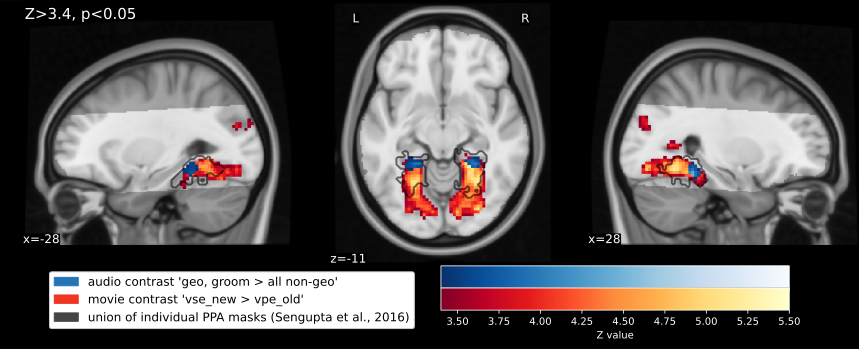
\includegraphics[width=\linewidth]{figures/group-slices}

    \caption{Mixed-effects group-level (N=14) clusters ($Z$>3.4, $p$<.05
      cluster-corrected) of activity correlated with the processing of spatial
      information are displayed on top of the MNI152 T1-weighted head template,
      with the acquisition field-of-view for the audio-description study
      highlighted.
      %
      The results of the audio-description's primary $t$-contrast (blue) that
      compares geometry-related nouns spoken by the narrator to non-spatial
      nouns (\texttt{geo, groom} > all non-spatial categories) are overlaid
      on the movie's primary $t$-contrast (red) that compares cuts to a
      setting depicted for the first time with cuts within a recurring setting
      (\texttt{vse\_new > vpe\_old}).
      %
      For comparison, the union of the individual PPA localization reported
      by \cite{sengupta2016extension} are indicated as a black outline.
    }

    \label{fig:group-slices}
\end{figure*}


\begin{table*}[tbp]
\caption{Clusters ($Z$-threshold $Z$>3.4; $p$<.05 cluster-corrected)
    of the primary $t$-contrast for the audio-visual movie comparing cuts to a
    setting depicted for the first time with cuts within a recurring setting
    (\texttt{vse\_new > vpe\_old}), sorted by size.
    The first brain structure given contains the voxel with the maximum $Z$-value,
    followed by brain structures from posterior to anterior, and partially
    covered areas (l.: left; r: right; c.: cortex; g.: gyrus; CoG: Center of
  Gravity).}
\label{tab:res-av-group1}
\small
\begin{tabular}{rrrrrrrrrp{4.7cm}}
\toprule
& & & \multicolumn{3}{r}{Max (MNI)} & \multicolumn{3}{r}{CoG (MNI)} &
\\ \cmidrule{4-6} \cmidrule{7-9}
Voxels & $p_{corr.}$ & $Z_{max}$ & X & Y & Z  & X & Y & Z & Structure \\
\midrule
3003 & <.00001 & 5.31 & 22.5 & -45.5 & -12 & 4.53 & -63.3 & -3.7 & r.~lingual g.; r.~cuneal c., intracalcarine c., bilaterally occipital fusiform g., precuneus,temporal fusiform c., posterior parahippocampal c.  \\
154 & <.00001 & 4.46 & -35 & -83 & 28 & -32.8 & -86.2 & 21.4 & l.~superior
lateral occipital c. \\ % 0.000000656
121 & <.00001 & 4.65 & 25 & -80.5 & 25.5 & 23.7 & -83.8 & 25.4 & r.~superior
lateral occipital cortex \\ % 0.00000769
\bottomrule
\end{tabular}
\end{table*}


% table group results primary AD contrast
\begin{table*}[tbp]
\caption{Clusters ($Z$-threshold $Z$>3.4; $p$<.05 cluster-corrected)
    of the primary $t$-contrast for the audio-description comparing
    geometry-related nouns to non-spatial nouns spoken by the
    audio-description's narrator (\texttt{geo, groom > all non-geo}), sorted by size.
    The first brain structure given contains the voxel with the maximum $Z$-value,
    followed by brain structures from posterior to anterior, and partially
    covered areas (l.: left; r: right; c.: cortex; g.: gyrus; CoG: Center of
    Gravity).}
    \label{tab:res-ao-group1}
\small
\begin{tabular}{rrrrrrrrrp{4.7cm}}
\toprule
& & & \multicolumn{3}{r}{Max (MNI)} & \multicolumn{3}{r}{CoG (MNI)} &
\\ \cmidrule{4-6} \cmidrule{7-9}
Voxels & $p_{corr.}$ & $Z_{max}$ & X & Y & Z  & X & Y & Z & Structure \\
\midrule
188 & <.00001 & 4.48 & -17.5 & -65.5 & 25.5 & -14.7 & -59.1 & 15.2 & l.~precuneus \\ % 0.0000000596
164 & <.00001 & 4.47 & 17.5 & -58 & 23 & 15.6 & -55.6 & 16 & r.~precuneus;
\\ % 0.000000238
83 & .00013 & 4.48 & 27.5 & -43 & -17 & 27.2 & -41.1 & -14 & r.~occipito-temporal fusiform c.; posterior parahippocampal g. \\ % 0.000128
73 & .00031 & 3.93 & -22.5 & -43 & -12 & -23.9 & -43.6 & -11.2 & l.~lingual
g.; occipito-temporal fusiform g., posterior parahippocampal c. \\ % 0.000128
63 & .00082 & 4.1 & 40 & -75.5 & 30.5 & 40.9 & -76.3 & 28.6 & r.~superior
lateral occipital c. \\ % 0.000824
37 & .0129 & 4.24 & -37.5 & -78 & 33 & -38.4 & -79.5 & 28.9 & l.~superior
lateral occipital c. \\ % 0.0129
\bottomrule
\end{tabular}
\end{table*}


\subsection{individual results}

% results in detail voxels of significant clusters in PPA ROI (and RSC
% liberally)
% sub-01 (m): PPA (l/r), AD (l/r), AV (-/r); RSC: AD (l/r), AV (-/-)
% sub-02 (m): PPA (l/r), AD (-/-), AV (l/-); RSC: AD (-/-), AV (-/-)
% sub-03 (f): PPA (l/r), AD (-/-), AV (-/r); RSC: AD (-/-), AV (-/-)
% sub-04 (f): PPA (-/r), AD (l/r), AV (-/r); RSC: AD (l/r), AV (-/-) !
% sub-05 (m): PPA (l/r), AD (-/-), AV (-/-); RSC: AD (-/-), AV (-/-)
% sub-06 (m): PPA (l/r), AD (l/r), AV (-/-); RSC: AD (l/-), AV (-/-)
% sub-09 (m): PPA (l/r), AD (l/-), AV (l/r); RSC: AD (l/r), AV (l/r)
% sub-14 (f): PPA (l/r), AD (l/r), AV (-/r); RSC: AD (l/r), AV (-/-)
% sub-15 (m): PPA (l/r), AD (l/r), AV (-/r); RSC: AD (l/r), AV (l/r)
% sub-16 (m): PPA (l/r), AD (l/r), AV (l/r); RSC: AD (l/r), AV (l/-)
% sub-17 (m): PPA (l/r), AD (l/r), AV (l/r); RSC: AD (l/r), AV (l/r)
% sub-18 (m): PPA (l/r), AD (l/r), AV (l/r); RSC: AD (l/r), AV (-/r)
% sub-19 (f): PPA (l/r), AD (l/r), AV (-/r); RSC: AD (l/r), AV (l/r)
% sub-20 (f): PPA (-/r), AD (-/-), AV (l/r); RSC: AD (-/-), AV (-/-)

% intro
Third, we inspected results from both naturalistic paradigms on the level of
individual participants, and compared them to the individual PPA localizations
provided by \cite{sengupta2016extension}, who reported
% Sengupta et al., 2016; unilateral in sub-04 and sub-20
bilateral parahippocampal clusters in 12 of 14 participants and unilateral right
clusters in two participants \citep[Tab.~3 in][]{sengupta2016extension}.
% one contrast to localize them all; "...and $Z$>3.4 for all"
Unlike \cite{sengupta2016extension}, who determined PPA clusters using three
candidate contrasts and a variable threshold, we used a single contrast for each
naturalistic stimulus and a uniform threshold for all participants.
% ref to figure
Figure~\ref{fig:subs-thresh-ppa} depicts thresholded $Z$-maps of the primary
movie and audio-description $t$-contrasts, in comparison to the results of a
conventional block-design localizer (unthresholded $Z$-maps are provided at
NeuroVault).
% AV
Results of the primary movie contrast yielded bilateral clusters in five
participants, a unilateral right cluster in six participants (of which one
participant yielded a unilateral cluster in the visual localizer), and a
unilateral left cluster in one participant.
% difference to dedicated localizer
We find bilateral clusters for participant \texttt{sub-20}, whereas the
block-design localizer yielded only one cluster in the right hemisphere.
% report here in group
Results of the primary audio-description contrast yielded bilateral clusters in
nine participants that are within or overlapping with the block-design localizer
results.
% subj-04
In participant \texttt{sub-04}, two bilateral clusters are apparent, whereas
block-design localizer, and movie stimulus yielded only one cluster in the right
hemisphere.
% sub-09
For another participant (\texttt{sub-09}) the analysis yielded one cluster in
the left-hemispheric PPA.


\begin{figure*}[tbp]
\centering
    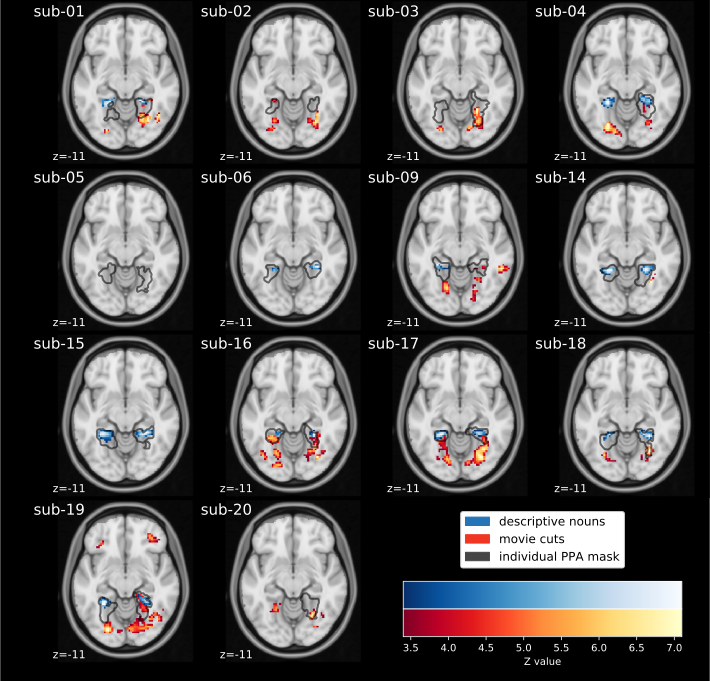
\includegraphics[width=\linewidth]{figures/subs-thresh-ppa}
    \caption{Fixed-effects individual-level GLM results ($Z$>3.4, $p$<.05
        cluster-corrected).
        Individual brains are aligned via non-linear
        transformation to a study-specific T2* group template that is
        co-registered to the MNI152 template with an affine transformation (12
        degrees of freedom).
        The results of the audio-description's primary
        $t$-contrast (blue) that compares geometry related nouns to non-
        geometry related nouns spoken by the narrator
        (\texttt{geo, groom > all non-geo}) are overlaid over the movie's
        primary $t$-contrast (blue) that compares cuts to setting depicted for
        the first time with cuts within a recurring setting
        (\texttt{vse\_new > vpe\_old}).
        Black:
        outline of participant-specific PPA ROIs.
        Light gray: The
        audio-description's field of view (cf. \citep{hanke2014audiomovie}).
        To facilitate comparisons across participants, we chose the same horizontal
        slice (x=-11) for all participants as this slice depicts voxels of
        significant clusters in almost all participants.
        The figure does not show voxels of the left cluster of the movie stimulus
        in sub-09 and sub-18, and voxels of the right cluster of the movie
        stimulus in sub-15.}
    \label{fig:subs-thresh-ppa}
\end{figure*}


\todo[inline]{SE: imo, key question is only partially answered: how close is
movie / audio to localizer". Can you corroborate figure 3 with some more
numbers? COH: schwierig vergleichbar (insb. unterschiedliche thresholds), daher
Bland-Altman-Plots -> as kinda mentioned in following paragraph}

% Bland-Altman-Plots
To illustrate the similarity of correlates of spatial processing in
naturalistic (audio-description) and conventional stimulation, independent of a
particular cluster-forming threshold, Bland-Altman plots for all participants
are shown in Figure~\ref{fig:bland-altman}.
% what it depicts
Each subplot visualizes the mean value and difference (localizer minus
audio-description) of all voxels in temporal and occipital cortices.
% maringal distributions
The marginal distributions of the mean scores indicate a general agreement of
both contrast scores across voxels in the PPA localization overlap as a
probabilistic indicator (blue), and the individual block-design localizer
results (red).
% lower right quadrant
Notably, 11 participants exhibit a pattern of increased $Z$-scores for the
naturalistic stimulus (lower right quadrant) that includes voxels labeled by the
block-design localizer, but also additional voxels.

\begin{figure*}[tbp]
\centering
    \includegraphics[scale=0.27]{figures/subjs_bland-altman.png}
    \caption{Bland-Altman-Plots for individual participants.
    The x-axes show the means of two spatially corresponding voxels in the
    unthresholded $Z$-map of the audio-description's primary contrast and
    unthresholded $Z$-map of the visual localizer (KDE plot on the top).
    The y-axes show the difference of two voxels (localizer minus
    audio-description; KDE plot on the right).
    The overlays depict voxels spatially constrained to the
    temporal and occipital cortex (gray; based on probabilistic Jülich
    Histological Atlas \citep{eickhoff2005toolbox, eickhoff2007assignment}),
    PPA overlap of all participants (blue),
    and individual PPA(s) (red).}
    \label{fig:bland-altman}
\end{figure*}


\section{Discussion}

% Discussion: explains how results fill gap identified in intro

% typically done by recapitulating the results, discussing limitations, and then
% revealing how the central contribution may catalyze future
% progress

% provides caveats to the interpretation describes how the paper
% advances the field by providing new opportunities

\todo[inline]{SE: mit Befund, den Du diskutieren willst beginnen, mit take-home
message enden. COH: bekomme ich nur (und auch nur evtl.) reingepresst, wenn ich
die Discussion komplett umschreibe; take-home message ist aber eh fast überall
drin}

\todo[inline]{SE: es gibt schon andere "event-related" analysen von movies,
oder? COH: habe Paper durchgeguckt: Es gibt wenig bis gar nichts (obwohl
Annotation immer mehr automatisiert werden können); Bzgl. Narrative ist im
Grunde alles "voxel-wise enconding"; Rocca benutzt Annotation, aber auch
"crafted" 23-min Narrative; NeuroScout: bisher absolut (?) keine veröffentlichte
Studie, die NeuroScout genutzt hat; -> Bartels ist Klassiker, steht aber enorm
allein da, und macht aber genau das, was wir machen "Naturalistic Stimulus statt
Traditionell"; insofern: es gibt schon "irgendwie" andere Studien, die etwas mit
Annotation (von Filmen) gemacht haben, die machen aber dann halt auch ganz
anderes Zeug}


%#1 previous studies
Several studies have reported increased hemodynamic activity in the PPA
attributed to the processing of spatial information, for example, when
participants were watching static pictures of landscapes compared to pictures of
faces or objects \citep[e.g.,][]{epstein1998ppa, epstein1999parahippocampal}.
% auditory semantics unclear
However, reports regarding the correlates of processing spatial information in
verbal stimulation are less clear \citep{aziz2008modulation}.
% current study: similar
In line with previous studies, we investigated the hemodynamic response to
spatial information using a model-based, mass-univariate approach.
% current study: dissimilar
However, instead of using a conventional set of stimuli, assembled to
specifically and predominantly evoke the processing of spatial information, we
employed a naturalistic stimuli, a movie and its audio-description, that were
designed for entertainment.

%#3 hypo
We hypothesized that due to the complex nature of the stimuli, unrelated factors
would be balanced across a large number of events, and make the bias of spatial
information accessible to a conventional model-based statistical analysis of BOLD
fMRI data.
% we need a detailed description -> annotation
This model-driven approach required a detailed annotation of the occurrence of
relevant stimulus features.
% event counts ftw
The annotation of both stimuli revealed the respective number of incidentally
occurring events to be similar to those of a conventional experimental paradigm
used to localize functional regions of interest.

%#4
We modeled hemodynamic responses correlating with spatial information embedded
in the naturalistic stimuli, capitalizing on conceptually similar, but
perceptually different stimulation events.
% group AV
On a group-average level, results for the movie show significantly
increased hemodynamic activity spatially overlapping with a conventionally
localized PPA but also extending into earlier visual cortices.
% group AD
Likewise, results for the audio-description identify significant activation in
the PPA but restricted to its anterior part.
% individual level
Bilateral clusters in 9 of 14
participants (of which \texttt{sub-04} shows only a right-lateralized PPA ROI
in the block-design localizer results), and a unilateral
significant cluster in one participant, indicate that the group average results
are representative for the majority of individual participants.
% meaning: generalization to naturalistic stimuli
These findings suggest that increased activation in the PPA during the
perception of static pictures generalizes to the perception of spatial
information embedded in a movie or a purely auditory narrative.
%
Current results may partially deviate from \cite{sengupta2016extension}, due to
the uniform cluster forming threshold employed in this study versus their
adaptive procedure (bilateral clusters in 12 of 14 participants and a unilateral
right cluster in two participants (\texttt{sub-04}, \texttt{sub-20}).

%#11 question
The fact that clusters from the auditory stimulus are spatially restricted to
the anterior part of clusters from both visual paradigms raises the question if
the revealed correlation patterns can be attributed to different features
inherent in the visual stimuli compared to a purely auditory stimulus.
% visual scenes: probably submodules
In the domain of visual scene perception, previous studies provide evidence
that the PPA can be divided into functionally subregions that might process
different stimulus features.
% posterior: functionality
The posterior PPA (pPPA) is functionally more responsive than the anterior PPA
(aPPA) to low-level features of scenes or (abstract) objects
\citep{baldassano2013differential, lescroart2019human, nasr2014thinking,
rajimehr2011parahippocampal}.
% anterior cIPL is defined using the Eickhoff–Zilles PGp probabilistic
% cytoarchitectonic map
In contrast, the aPPA responds more to high-level features of scenes (e.g.
real-word size \citep{park2015parametric}; a scene's abstract category
\citep{marchette2015outside, watson2016patterns}) and objects (e.g. spatial
contextual associations \citep{aminoff2007parahippocampal, aminoff2013role})
than the pPPA.
% connectivity
Moreover, pPPA and aPPA show differences in connectivity profiles.
% posterior
The pPPA exhibits more coactivation with the occipital visual cortex than the
aPPA \citep{baldassano2013differential, baldassano2016two}.
% including lateral occipital cortex (LOC) and transverse occipital sulcus
% (TOS) anterior
Activity in the aPPA, on the other hand, is found to be correlated with
components of the default mode network, including caudal inferior parietal lobe,
retrosplenial complex, medial prefrontal cortex, and lateral surface of
the anterior temporal lobe \citep{baldassano2013differential,
baldassano2016two}.\todo{last half sentence is almost a direct quote;
plagiarism?}
% conclusion: subregions
\cite{baldassano2013differential} proposes that the PPA creates a complete
scene representation, based on different aspects of a visual scene processed in
subregions of the PPA.
% Their distinct connectivity properties do suggest that each may be involved
% in specific aspects of visual and cognitive processing involved in the
% overarching goal of scene understanding \citep{baldassano2013differential}.
% The fact that anterior PPA had a lower sensitivity to our abstract object
% stimuli does not necessarily imply that this region does not use object
% information \citep{baldassano2013differential}. Previous work has shown that
% PPA responds to objects that have spatial associations [Aminoff et al. 2007],
% are space-defining [Mullally and Maguire 2011], and are
% navigationally-relevant [Janzen and Van Turennout 2004]. These types of
% responses require spatial memory and cannot be based purely on visual
% features like object shape. \citep{baldassano2013differential}.  pPPA
Similarly, our results suggest that the pPPA is more concerned with visual
aspects immanent in pictures or movie shots of landscapes.
% aPPA
The aPPA might be more concerned with non-visual aspects of spatial information
(e.g. spatial contextual information \citep{aminoff2007parahippocampal}) as
immanent in both visual and verbal stimuli.


%#6 hypothesis
Based on the report by \cite{aziz2008modulation}, we hypothesized that semantic
spatial information embedded in the audio-description would correlate with
increased hemodynamic activity in the PPA.
%
Methods and results presented here differ from this previous study in key
aspects.
% diff to Aziz (2008)
\cite{aziz2008modulation} modeled events from onset to offset of sentences,
describing unknown and famous places and faces, and compared activity levels
that were averaged across voxels of ROIs (PPA and fusiform face area, FFA
\citep{kanwisher1997ffa}) defined by a localizer experiment.
% Aziz results
Their results showed decreased activity in only the left PPA
compared to activity in the FFA for sentences describing famous places in contrast
to famous faces.
% we: model & whole brain
Here, we modeled events from onset to offset of single words and performed a
voxelwise whole-brain analysis.
% our results
Group results of the audio-description's primary contrast yielded significantly
increased hemodynamic activity spatially restricted to the anterior part of the
PPA group overlap.
% concluding statement
Contrary to \cite{aziz2008modulation}, our results suggest that auditory
spatial information compared to non-spatial information correlates with
bilaterally increased activation in the anterior part of the PPA.

%#7 previous studies: no task
It is common for conventional localizer paradigms to employ a task to keep
participants attentive to the stimuli.
% but: Epstein (1998)
Nevertheless, one early block-design study \citep{epstein1998ppa} compared
results from a paradigm that employed a perceptual judgment task of static
pictures to the same paradigm but without that task.
% results during no task
Hemodynamic activity was less but still significantly increased when
participants had no task to keep them alert and attentive to the stimuli.
% we have no task neither
The naturalistic stimulation paradigm employed here is similar in the sense that
participants had no behavioral or cognitive task \cite[e.g., forming a mental
image of the stimuli;][]{ocraven2000mental} but just had to ``enjoy the
presentation''.
% but still: we are different
Nevertheless, the naturalistic paradigm differs from \cite{epstein1998ppa},
because the relevant stimulus features were embedded in a continuous stream of
complex auditory (and visual) information which makes it unlikely that
participants speculated on the purpose of the investigation, or performed
undesired and unknown evaluation or categorization of isolated stimuli.
% concluding statement: kinda automatic process
Our results therefore indicate that verbally communicated spatial information is
processed, in the anterior PPA, automatically and without specifically guided
attention.


% shortcomings
%#2
Our approach to stimulus annotation and event selection differs from previous
reports in the literature.
% PPA: intro
In an earlier study, \cite{bartels2004mapping} manually annotated the content of
movie frames (color, faces, language, and human bodies) and found that the
functional specialization of brain areas is preserved during movie watching.
%
In contrast, we aimed to exploit a cinematographic confound in the structure of
movies, where
% establishing shots vs. e.g. over-the-shoulder shots
film directors tend to establish the spatial layout of locations in earlier
shots and later focus more on detailed depictions of people and objects
\citep{brown2012cinematography, katz1991film, mascelli1998five}.
% results
The group results of the movie stimulus' primary contrast yielded a large
cluster that spans the group overlap of individual PPA ROIs from anterior to
posterior.
% confound of higher perception
The cluster extends into more posterior, earlier visual areas could be an
indication that the temporal averaging across events suffered from insufficient
controlling for confounding visual features.
% solution
Future studies that aim to use a movie to localize visual areas in individual
participants should extensively annotate the content of frames \citep[e.g.,
using the open-source solution ``Pliers'' for feature extraction from a visual
naturalistic stimulus;][]{mcnamara2017developing}.

%#8
% optimal stimulus type in vision
In the visual domain, pictures of landscapes and not pictures of landmarks or
buildings are considered to be the ``optimal'' stimulus type
\citep{epstein2008parahippocampal}.
% we did not choose se\_new and se\_old
In the audio-description's primary contrast, we did not include the categories
that contain switches from one setting to another (\texttt{se\_new} and
\texttt{se\_old}) which one might assume to contain the auditory equivalent to
pictures of landscapes.
% why
The reason was that the categories \texttt{se\_new} and \texttt{se\_old} were
heterogeneous: they rarely contained holistic (but also vague) descriptions of
landscapes (e.g.  ``[Forrest is running through the] jungle'') but mostly
landmarks or buildings, and also non-spatial hints (e.g. ``[Jenny as a]
teenager``).
% visual system => gist in milliseconds
Humans can identify the gist of a rich visual scene within the duration of a
single fixation \citep{henderson2003human}.
%
Hence, further studies might investigate if vague verbal descriptions of
landscapes lead to a different hemodynamic activity level than descriptions of
more concrete parts of a scene (e.g.``[a] beacon'', [a] ``farmhouse'').
%#5


% MIH: second time this notion is coming up in the discussion
%% we took advantage of cinematography
%We here took advantage of an idiosyncrasy of movie directing to shift from
%depicting the spatial layout to to later depicting persons and objects.
%% know your stimulus
%Given that this shift is common in movies, investigators should be aware that
%cinematographic tendencies are part of movie's confound structure that might,
%depending on the research question, influence the results.
%% conclusion
%In summary, results from the visual localizer paradigm using blocks of pictures
%generalize to an ad hoc approach to operationalize the perception of spatial
%information at the moment of cuts in an audio-visual movie.

%#12 RSC + LOC
Apart from the PPA, results show significantly increased activity in the dorsal
precuneus and posterior cingulate region (e.g. retrosplenial complex; RSC) and
lateral occipital cortex (LOC; more lateral in the movie stimulus, more medial
in the audio-description stimulus) for both naturalistic stimuli.
% RSC intro
Like the PPA, the RSC and LOC repeatedly exhibited increased hemodynamic
activity in studies investigating visual spatial perception or navigation (see
\citep{chrastil2018heterogeneity, bettencourt2013role, epstein2019scene} for
reviews)
% not random shit
Thus, our model-driven approach to operationalize spatial perception based on
stimulus annotations reveals focussed activation patterns in networks that are
implicated in visual spatial perception and cognition.

%#13 natural stimulation
In summary, natural stimuli like movies \citep{eickhoff2020towards,
hasson2008neurocinematics, sonkusare2019naturalistic} or narratives
\citep{hamilton2018revolution, honey2012not, lerner2011topographic,
silbert2014coupled, wilson2008beyond} can be used as a continuous, complex,
immersive, task-free paradigm that more closely resembles our natural dynamic
environment than traditional experimental paradigms.
% method
We took advantage of three fMRI datasets and two stimulus annotations that are
part of the open-data resource
\href{http://www.studyforrest.org}{studyforrest.org} to operationalize the
perception of spatial information embedded in an audio-visual movie and an
auditory narrative, and compare current results to a previous report of a
conventional, block-design localizer.
% results
The current study offers evidence that a model-driven GLM analysis based on
annotations can be applied to a naturalistic paradigm to localize concise
functional areas and networks correlating with specific perceptual processes.
% interpretation
More specifically, our results demonstrate that increased activation in the PPA
during the perception of static pictures generalizes to the perception of
spatial information embedded in a movie and an exclusively auditory stimulus.
% interpretation: aPPA vs. pPPA
Our results provide further evidence that the PPA can be divided into
functional subregions that coactivate during the perception of visual scenes.
% interpretation
Finally, the presented evidence on the in-principle suitability of a naturally
engaging, purely auditory paradigm for localizing the PPA may offer a path to
the development of diagnostic procedures more suitable for individuals with
visual impairments or conditions like nystagmus.

\todo[inline]{SE: mir das Potential (warum ist das relevant -> rich stimulus ie
many possible analyses, better compliance, easier to perform for difficult
populations, etc) eigentlich zu kurz; COH: finde ich (insb. als allerletzten)
Satz in einem Satz so okay, weil a) Textlimit, b) exploratory \& <80 \%
lokalisationsleistung; wenn, dann müsste man ein größeres Fass in Intro und
Discussion aufmachen, was die Ergebnisse aber nicht hergeben }


\subsection*{Data and code availability}

% Zenodo (registered but zipped) vs. OSF (datalad dataset but probably
% unregistered)
The fMRI and annotation data, analysis scripts to generate the results as well
as results are available in the gin repository,
\href{https://gin.g-node.org/chaeusler/studyforrest-ppa-analysis}{gin.g-node.org/chaeusler/studyforrest-ppa-analysis}, accessible as Datalad (RRID:SCR\_003931) datasets.


\section*{Acknowledgements}

\todo[inline]{everything correct? Grant or contribution numbers may be acknowledged}
%
COH designed and performed the analyses, and wrote the manuscript.
%
MH provided critical feedback on the procedure and edited the manuscript.
%
SE provided critical feedback.
%
We are grateful to \href{www.florianschurz.de}{Florian Schurz} who initiated the
annotation of nouns and created its preliminary version.%

This research was, in part, supported by the German Federal Ministry of
Education and Research (BMBF, 01GQ1112) and the US National Science Foundation
(NSF, 1129855). Work on the data-sharing technology employed for this research
was supported by BMBF (01GQ1411, 01GQ1905) and NSF (1429999, 1912266).

\section*{Competing financial interests}
The authors declare no competing financial interests.


{\small\bibliographystyle{unsrtnat}
\bibliography{references}}

%\begin{thebibliography}{1}
%\expandafter\ifx\csname url\endcsname\relax
%  \def\url#1{\texttt{#1}}\fi
%\expandafter\ifx\csname urlprefix\endcsname\relax\def\urlprefix{URL }\fi
%\providecommand{\bibinfo}[2]{#2}
%\providecommand{\eprint}[2][]{\url{#2}}
%
%\bibitem{cite1}
%\bibinfo{author}{Califano, A.}, \bibinfo{author}{Butte, A.~J.},
%  \bibinfo{author}{Friend, S.}, \bibinfo{author}{Ideker, T.} \&
%  \bibinfo{author}{Schadt, E.}
%\newblock \bibinfo{title}{{Leveraging models of cell regulation and GWAS data
%  in integrative network-based association studies}}.
%\newblock \emph{\bibinfo{journal}{Nature Genetics}}
%  \textbf{\bibinfo{volume}{44}}, \bibinfo{pages}{841--847}
%  (\bibinfo{year}{2012}).
%
%\bibitem{cite2}
%\bibinfo{author}{Wang, R.} \emph{et~al.}
%\newblock \bibinfo{title}{{PRIDE Inspector: a tool to visualize and validate MS
%  proteomics data.}}
%\newblock \emph{\bibinfo{journal}{Nature Biotechnology}}
%  \textbf{\bibinfo{volume}{30}}, \bibinfo{pages}{135--137}
%  (\bibinfo{year}{2012}).
%\end{thebibliography}


\section{Data Citations}

\begin{itemize}
% cut anno
\item Häusler, C. O. \& Hanke M. Dataset 1 in: An annotation of cuts, depicted
locations, and temporal progression in the motion picture "Forrest Gump".
\emph{F1000Research}
\href{https://doi.org/10.5256/f1000research.9536.d134823}{10.5256/f1000research.9536.d134823}
(2016)

% speech anno
\item Häusler, C. O. \& Hanke M. \emph{OSF}
\href{https://doi.org/10.17605/OSF.IO/GFRME}{10.5256/f1000research.9536.d134823}
(2020).

% audio-description
\item Hanke, M., Baumgartner, F.~J., Ibe, P., Kaule, F.~R., Pollmann, S., Speck, O.,
  Zinke, W., \& Stadler, J. \emph{OpenfMRI} \href{https://openfmri.org/dataset/ds000113}{ds000113} (2014)

\item Sengupta, A., Kaule, F. R., Guntupalli, J. S., Hoffmann, M. B., Häusler, C., Stadler, J. \& Hanke, M.
  \emph{OpenfMRI} \href{https://openfmri.org/dataset/ds000113c}{ds000113c} (2016).

\item Hanke, M., Adelhöfer, N., Kottke, D., Iacovella, V., Sengupta, A., Kaule, F.~R., Nigbur, R., Waite, A.~Q.,
  Baumgartner, F.~J. \& Stadler, J. (2016).
  \emph{OpenfMRI} \href{https://openfmri.org/dataset/ds000113d}{ds000113d} (2016).
\end{itemize}


\appendix

\pagebreak[4]

\setcounter{figure}{0}
\makeatletter
\renewcommand{\thefigure}{S\@arabic\c@figure}
\makeatother

\section{Supplementary Materials}


\subsection{additional contrasts}

\todo[inline]{remove subheadings}

\todo[inline]{introductory \& concluding sentences}

\subsubsection{PPA, RSC, and LOC (AV \& AV)}

\todo[inline]{SE: use different colormap for overlap of contrasts' clusters}

\todo[inline]{I manually adjusted the stability-slices.pdf; the Fig S1 should
now (not just on my computer) show a black bar in the color maps for the
audio-descriptions (because there are 5 and not 8 contrasts)}

% intro
In order to test the robustness of our approach, we created overall five
$t$-contrasts for the movie stimulus, and overall eight $t$-contrast for the
audio-description (Tab.~\ref{tab:contrasts}).
% how
Contrasts differ in contrasted categories based on ``how well'' averaged events
within categories were considered to represent spatial and non-spatial
information, and the number of events in the stimulus.
% NeuroVault
Unthresholded $Z$-maps of all contrasts on a group level co-registered to the
group-template (MNI152 space) can found at
\href{https://neurovault.org/collections/KADGMGVZ/}{\url{neurovault.org/collections/KADGMGVZ}}.

% AV PPA contrasts
% 1 PPA (l/r); RSC (l/r), LOC (l/r), VisC (l/r),
% intracalcarine, cuneal, ling.c
% 2 PPA (l/r); RSC (-/-), LOC (l/r), VisC (-/-)
% 3 PPA (l/r); RSC (-/-), LOC (-/-), VisC (-/r), occ. fusisf. g.
% 4 PPA (l/r); RSC (l/r), LOC (l/r), VisC (-/-), lingual g., occ. fusif. g.
% 5 PPA (l/r); RSC (l/r), LOC (l/r), VisC (-/-), occ. fusif. g.

% AV results: PPA; biggest overlap in posterior part of PPA group overlap  =
% temporal occipital fusiform cortex
Reliably across all five movie contrasts, we find bilaterally significant
clusters that overlap with the PPA group overlap
(Fig.~\ref{fig:stability-slices}).
% AV: RSC & LOC
Several contrasts of the movie also yielded bilaterally significant clusters in
the ventral precuneal cortex and posterior cingulate gyrus (i.e. retrosplenial
complex; contrasts 1, 4, 5), and lateral occipital cortex (contrasts 1, 2, 4,
5).

% AD PPA contrasts
% 1 PPA (l/r); RSC (l/r), LOC (l/r)
% 2 PPA (l/r); RSC (l/r), LOC (l/r), r. sup.temp.C., r.fr.pole; putamen; etc
% 3 PPA (l/r); RSC (l/r), LOC (l/r),l&r sup.temp.C., anterior cing., paracing.
% 4 PPA (l/r); RSC (l/r), LOC (l/r)
% 5 PPA (l/r); RSC (l/r), LOC (-/-)
% 6 PPA (l/r); RSC (l/r), LOC (l/-), l&r sup.temp.C.; medial pref. c., precun
% 7 PPA (-/-); RSC (l/r), LOC (l/-), l&r sup.temp.C.; left frontal pole
% 8 PPA (-/-); RSC (-/-), LOC (-/-)

% AD: results
In results from the analysis of the audio-description, all contrasts except
contrast 7 and 8  yielded significant bilateral clusters in anterior regions of
the group PPA overlap (Fig.~\ref{fig:stability-slices}).
% AD: RSC & LOC
Contrasts of the audio-description also yielded bilaterally significant clusters
in the ventral precuneus (all contrasts except contrasts 8) and lateral
occipital cortex (bilateral in contrasts 1 to 4; unilateral in contrasts 6 and
7).
% concluding stament regarding PPA, RSC, and LOC
Results across contrasts of both naturalistic stimuli indicate that our findings
regarding the PPA but also RSC and LOC are robust and do not depend on the
design of one specific contrasts.
% but:
Nevertheless, results are sensitive to the contrasted categories and the amount
of available data.
% example
For example, contrast 7 and 8 (\texttt{se\_new}, \texttt{se\_old} > non-spatial
categories, and \texttt{se\_new} > non-spatial categories) that used the most
heterogeneous categories (nouns indicating switches to other settings) and a low
amount of events yielded neither a significant cluster in the right-hemispheric
nor left-hemispheric PPA.
% concluding statement
Hence, investigators that use model-driven analyses have to consider how many
events a naturalistic stimulus may provide and how homogeneous the events to be
averaged might be.


\subsubsection{auditory cortices}

Several contrasts yielded significant clusters in superior temporal cortices
(bilateral in contrasts 3, 6, 7; unilateral right in contrast 2).
% AD: auditory cortices
Further, contrasts that compare, possibly among others, nouns indicating a
switch to another setting (categories \texttt{se\_new} or \texttt{se\_old}) to
non-spatial categories yielded significant clusters in superior temporal
cortices (bilateral: contrasts 3, 6, 7; unilateral right: contrast 2).
% interpretation 1
This suggests that variance correlating with lower level auditory processes was
not averaged out across events and the employed nuisance regressors did not
capture this variance appropriately.\todo{this sounds shitty}
% interpretation 2
Another possibility might be that increased hemodynamic activity in superior
temporal cortices reflect a bias towards lower-level auditory perceptual
processes on the positive side of the GLM contrasts.
% soundscape
Increased activity in primary and secondary auditory cortices could be
attributed to changes in the soundscape that possibly accompany the narrator
when he is indicating the switch to another setting by describing its identity
or layout.\todo{speculative though}
% concluding statement
\todo[inline]{concluding statement?}



\subsubsection{``random clusters''}

\todo[inline]{following list is exhaustive but probably too detailed}
%
Lastly, contrasts of the audio-description stimulus yielded significant clusters
in regions that were statistically in two or less contrasts.
% contrast 2
In detail, contrast 2 yielded clusters in the anterior cingulate gyrus
(bilateral), right frontal pole, right frontal medial cortex, and right putamen.
% contrast 3
Contrast 3 shows clusters in the anterior cingulate gyrus (bilateral), left
frontal pole, and left insular.
% contrast 6
Contrast 6 shows one additional cluster in the right medial frontal cortex.
% contrast 7
Contrast 7 shows clusters in the left frontal pole and left frontal operculum,
left insular.
% concluding statement
Here again, significantly increased activation beyond areas known to be involved
in processing of spatial information can be attributed to stimulus features of
the naturalistic stimulus that were not sufficiently controlled leading to a
bias in the contrasts.
%
\todo[inline]{imo other interpretations would speculative / reverse inference;
but "if would look closer I would probably find a super plausible reason why
brain areas are more active"}


\begin{figure*}[tbp]
\centering
    \includegraphics[width=\linewidth]{figures/stability-slices}
    \caption{Overlap of significant clusters ($Z$>3.4; $p$<.05, cluster corrected)
        The audio-description's contrasts 1-8 (blue)
        are overlaid over the audio-visual movie's contrasts 1-5 (red;
        \ref{tab:contrasts}).
        Cluster are overlaid on top of the MNI152 T1-weighted head template
        with the acquisition field-of-view for the audio-description study
        highlighted.
        Black: outline of overlapping individual PPA ROIs.
        The figure shows that some contrasts yielded significant clusters
        also in the lateral temporal and prefrontal cortex.
        }
    \label{fig:stability-slices}
\end{figure*}


\subsection{Control contrasts}

\todo[inline]{This section feels incomplete. Some explanation (attempts) are
missing. Sometimes it is simply unclear which data were analyzed with which
designs. Maybe subheadings would help?}

% ---------- AV control contrasts ----------
% 6: nothing; 7 nothing; 8: nothing; 9: nothing; 10 se_new > se_old (nouns but
% in AV stimulus): LOC (l/r) right PPA, bilateral, sup. lat. occ. c., sup.
% parietal lobe (right)

% ---------- AD control contrasts ----------
% 9 PPA (-/-); RSC (-/r), LOC (-/-), left pars triangularis
%10 PPA (-/-); RSC (-/-), LOC (-/-)
%11 PPA (-/-); RSC (-/-), LOC (-/-),
%12 PPA (-/-); RSC (-/-), LOC (-/-), right posterior hippocampus
%13 PPA (-/-); RSC (-/-), LOC (-/-)

% intro
For each naturalistic stimulus, we created several control contrasts.
% movie contrasts: not cut condition vs. cuts
To test for XYZ\todo{yes, to test what?} within the movie fMRI data, we created
four contrasts that compared hemodynamic activity during frames within movie
shots (\texttt{no\_cut} category) with movie cut related categories
(Tab.~\ref{tab:contrasts}).
% results
None of these four contrasts yielded a significant cluster.
%
Null results of control contrasts comparing frames within movie shots to frames
immediately after a cut suggest that XYZ.
%
\todo[inline]{concluding statement}

% \texttt{se\_new} (nouns) is r$\approx$0.3 correlated with \texttt{vse\_new}
% (cuts); \texttt{se\_old} (nouns) is r$\approx$0.4 correlated with
% \texttt{vse\_old}.
The inspection of correlations of regressors across stimuli
(Fig.~\ref{fig:reg-corr}) showed a moderate correlation among cuts to a setting
depicted for the first time (\texttt{vse\_new}) and nouns indicating a switch to
a setting occurring for the first time (\texttt{se\_new}), and cuts to a
recurringly depicted setting ({\texttt{vse\_old}) and nouns indicating a switch
a recurring setting (\texttt{se\_old}.
%
Hence, we created a contrast that used the audio-description's nouns on the
movie data ({\texttt{se\_new} > \texttt{se\_old}).
% results
The contrasts yielded a significant cluster in the right [but not anterior] PPA
and bilateral clusters in the superior lateral occipital cortices (the right
hemispheric cluster extending into the superior parietal cortex).
%
Results suggest that XYZ.
%
\todo[inline]{concluding statement? That last contrast was originally done to
check that "soundscape at moment of cuts thing" but this is obsolete now}

\todo{following: control contrast for AO; why exactly did we do this except "we
do not expect (lots of) significant cluster because negative control?}

% AD stimulus
Finally for the analysis of the audio-description, we created control contrasts
based on events of the annotated movie cuts (Tab.~\ref{tab:contrasts}) in
order to test XYZ.
% results
Two of five contrasts yielded significant clusters.
% contrast 9
Contrast 9 (\texttt{vse\_new > pe\_old}) revealed one significant cluster in the
left inferior prefrontal cortex (pars triangularis) and right ventral
precuneus/posterior cingulate gyrus.
% contrast 12
Contrast 12 (\texttt{vse\_new} > \texttt{vse\_old}, \texttt{vpe\_old}) revealed
one cluster in the right posterior hippocampus.  \todo{not PPA! explanation?}
%
Overall results from the negative control contrast of the audio-description's
data suggest that XYZ.
%
\todo[inline]{concluding statement?}


\end{document}
